\chapter{Analisi Risultati}

\medskip
In questo capitolo si analizza in primo luogo quale approccio, tra approccio classico (\textit{classic}), approccio time series con media mobile (\textit{TS-MA}) e approccio time series con differenze (\textit{TS-Diff}), dimostra performance migliori, in termini di MCC, error rate e speed score. In secondo luogo, vengono discussi i risultati delle performance dei modelli sul dataset \textit{my-all3}. Per concludere si commentano i risultati differenti al variare dei parametri \textit{window} e \textit{shuffle}.

\section{Progressione MCC, Error Rate e Speed Score}
In questa sezione sono presentati i risultati, quindi i grafici, della progressione dell'MCC, dell'Error Rate e dello Speed Score. Come detto nel Capitolo 3, non \`e appropriato rimescolare i dati quando si tratta di dati time series, quindi per i risultati discussi in questa sezione il parametro \textit{shuffle} \`e sempre uguale a \textit{False}.
A seguire sono illustrati i grafici delle progressioni, partendo da una finestra temporale (\textit{window}) uguale a 5 arrivando fino a 2.
\begin{itemize}
    \newpage
    \item \textit{\textbf{window = 5}, shuffle = False}:
    \begin{figure}[H]
    \centering
    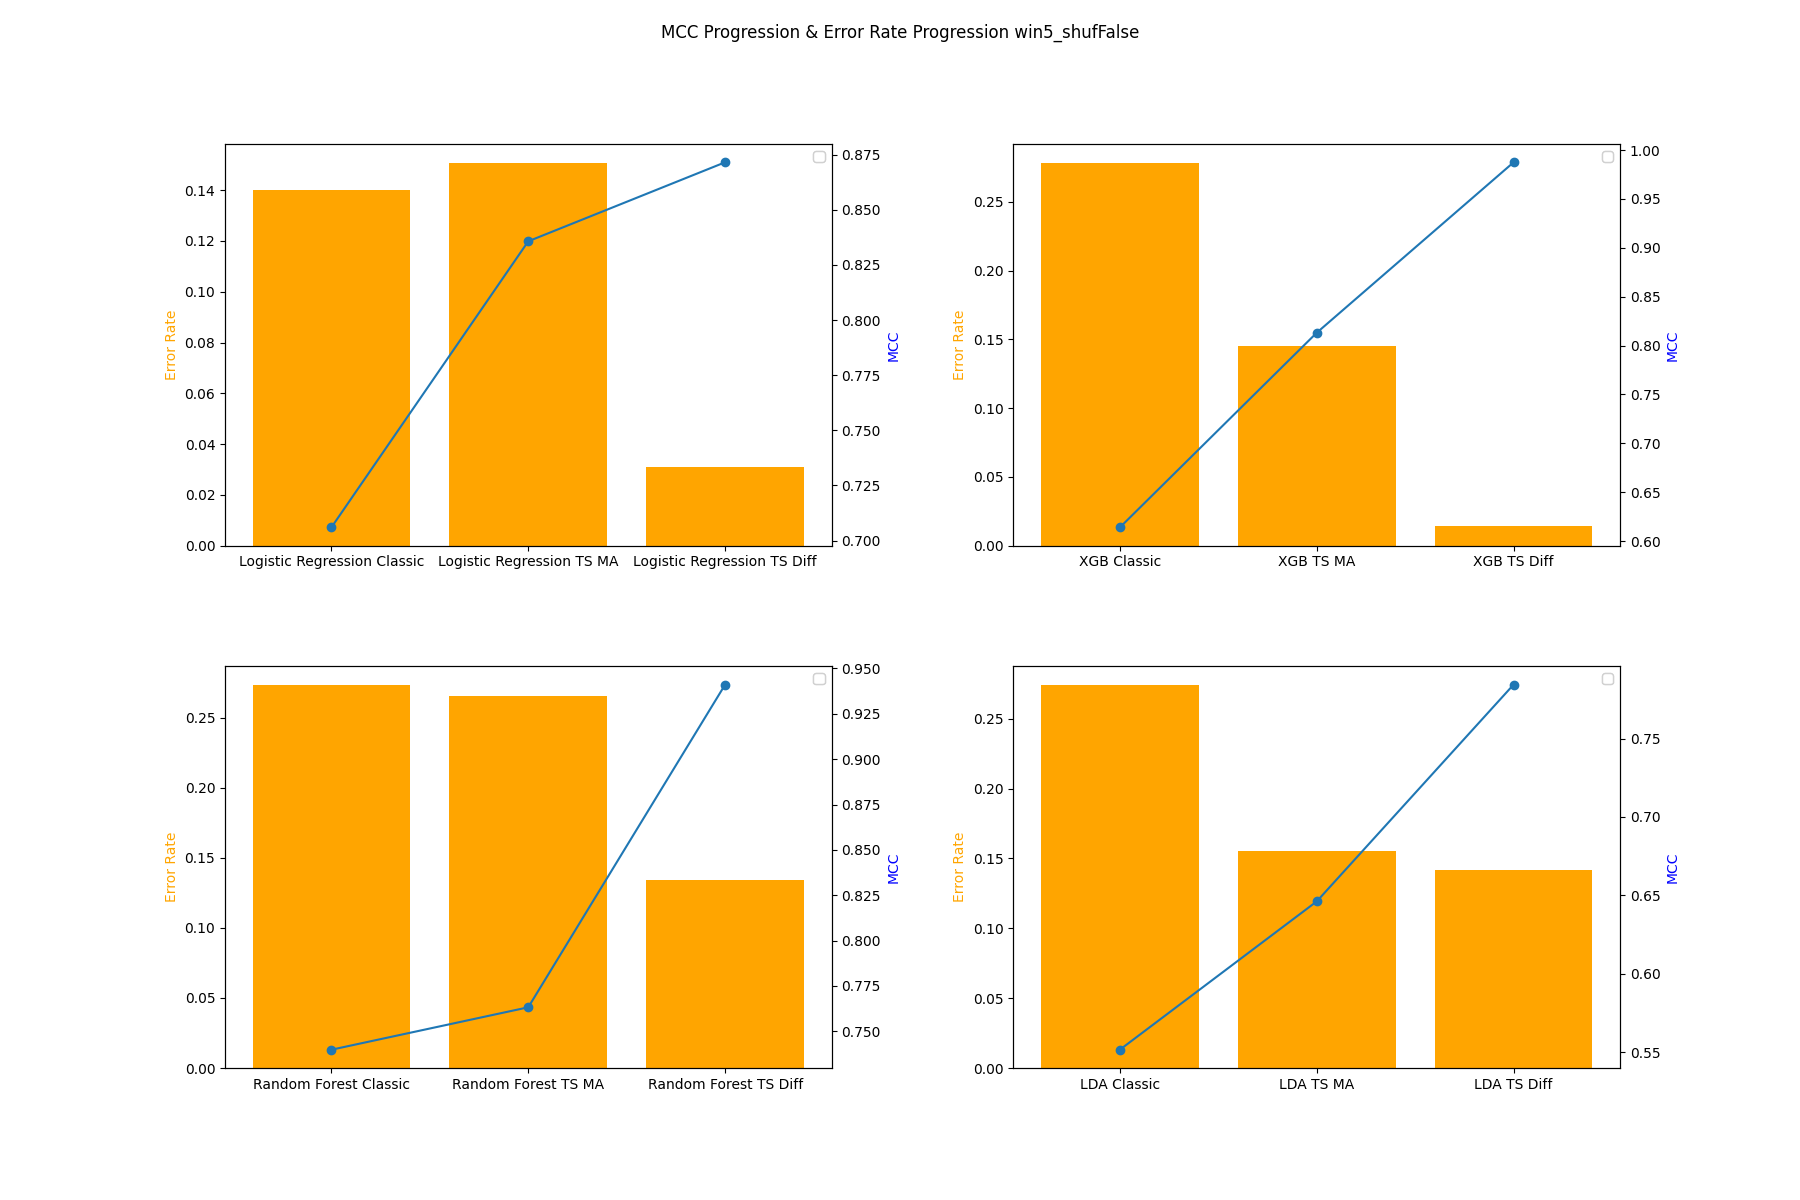
\includegraphics[width=0.94\linewidth]{MCC_Progression_win5_shufFalse.png}
    \caption{Progressione MCC ed Error Rate window=5,shuffle=False}
    \label{fig:enter-label}
    \end{figure}
    \begin{figure}[H]
    \centering
    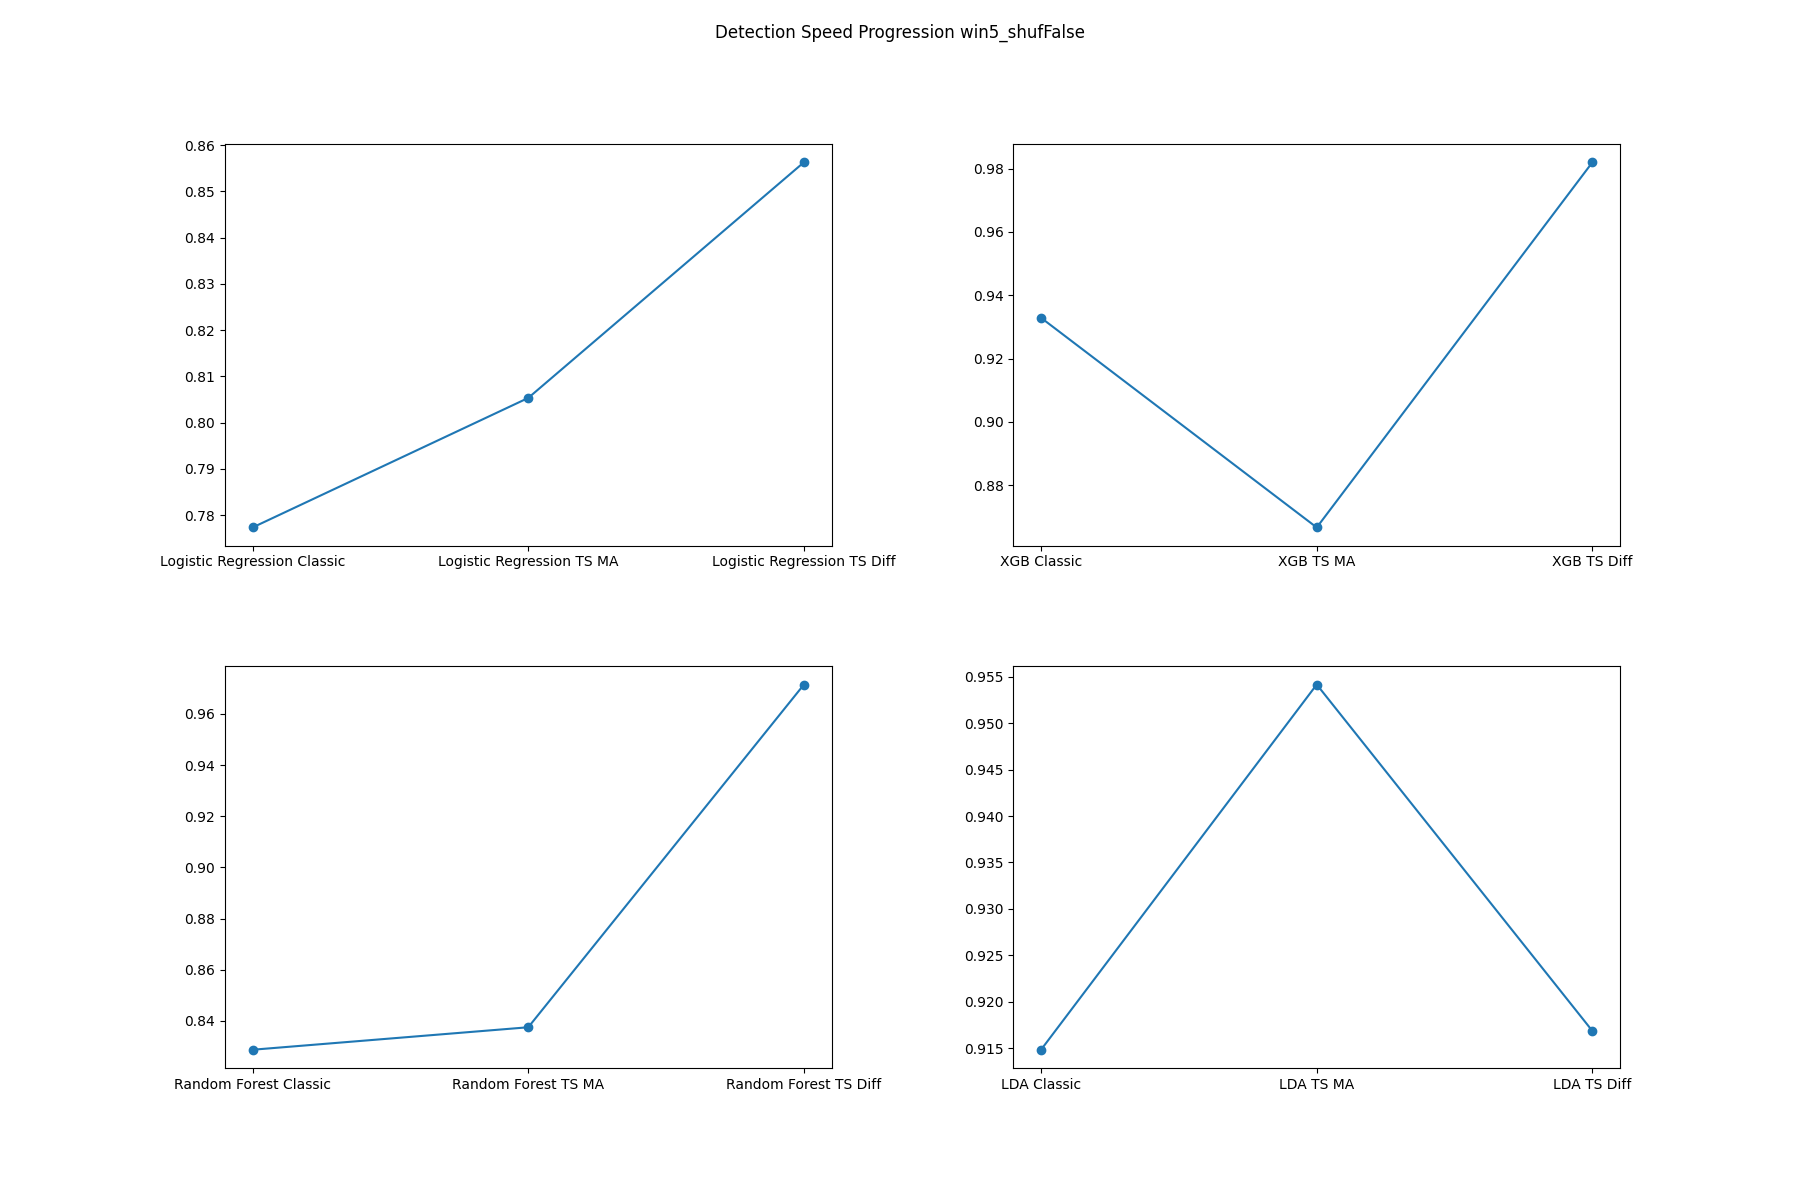
\includegraphics[width=0.94\linewidth]{Speed_Progression_win5_shufFalse.png}
    \caption{Progressione Speed Score window=5,shuffle=False}
    \label{fig:enter-label}
    \end{figure}

    \newpage
    \item \textit{\textbf{window = 4}, shuffle = False}:
    \begin{figure}[H]
    \centering
    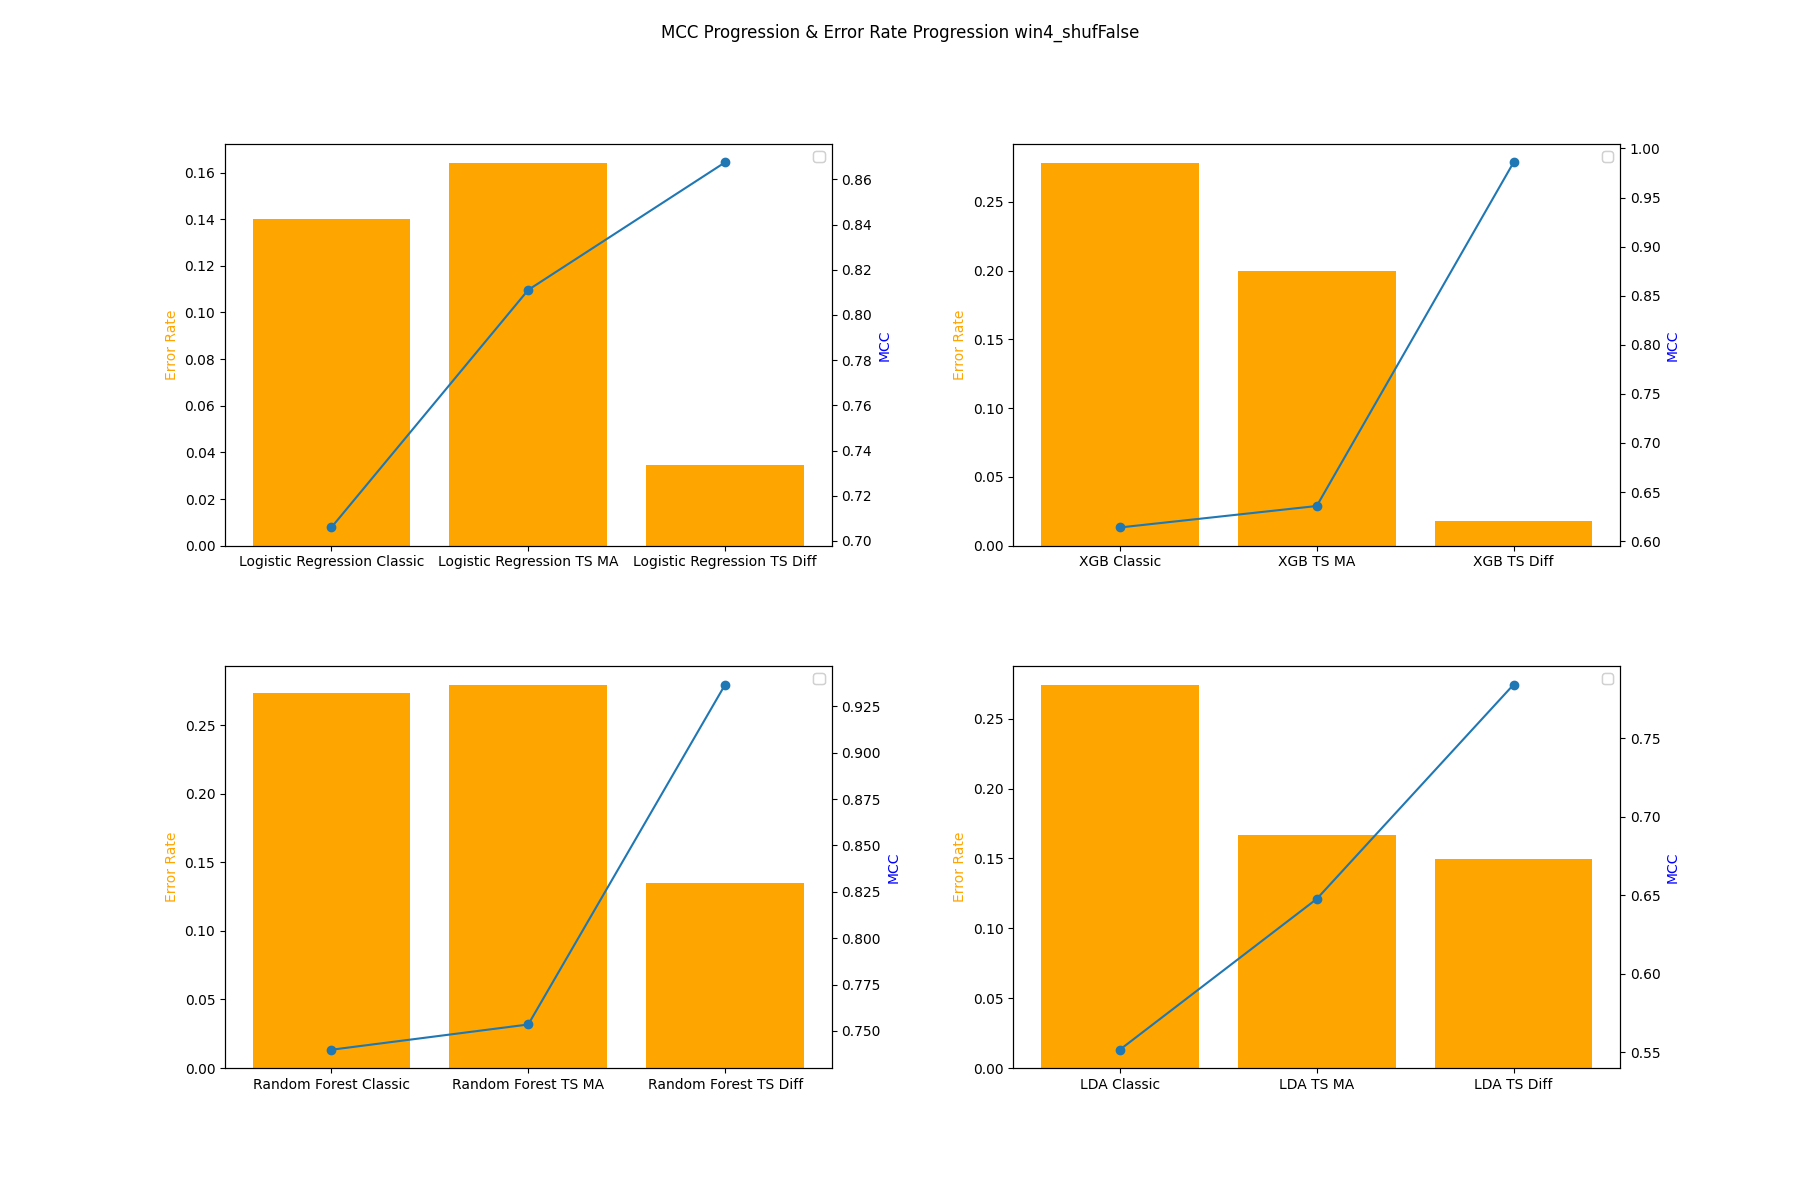
\includegraphics[width=0.94\linewidth]{MCC_Progression_win4_shufFalse.png}
    \caption{Progressione MCC ed Error Rate window=4,shuffle=False}
    \label{fig:enter-label}
    \end{figure}
    \begin{figure}[H]
    \centering
    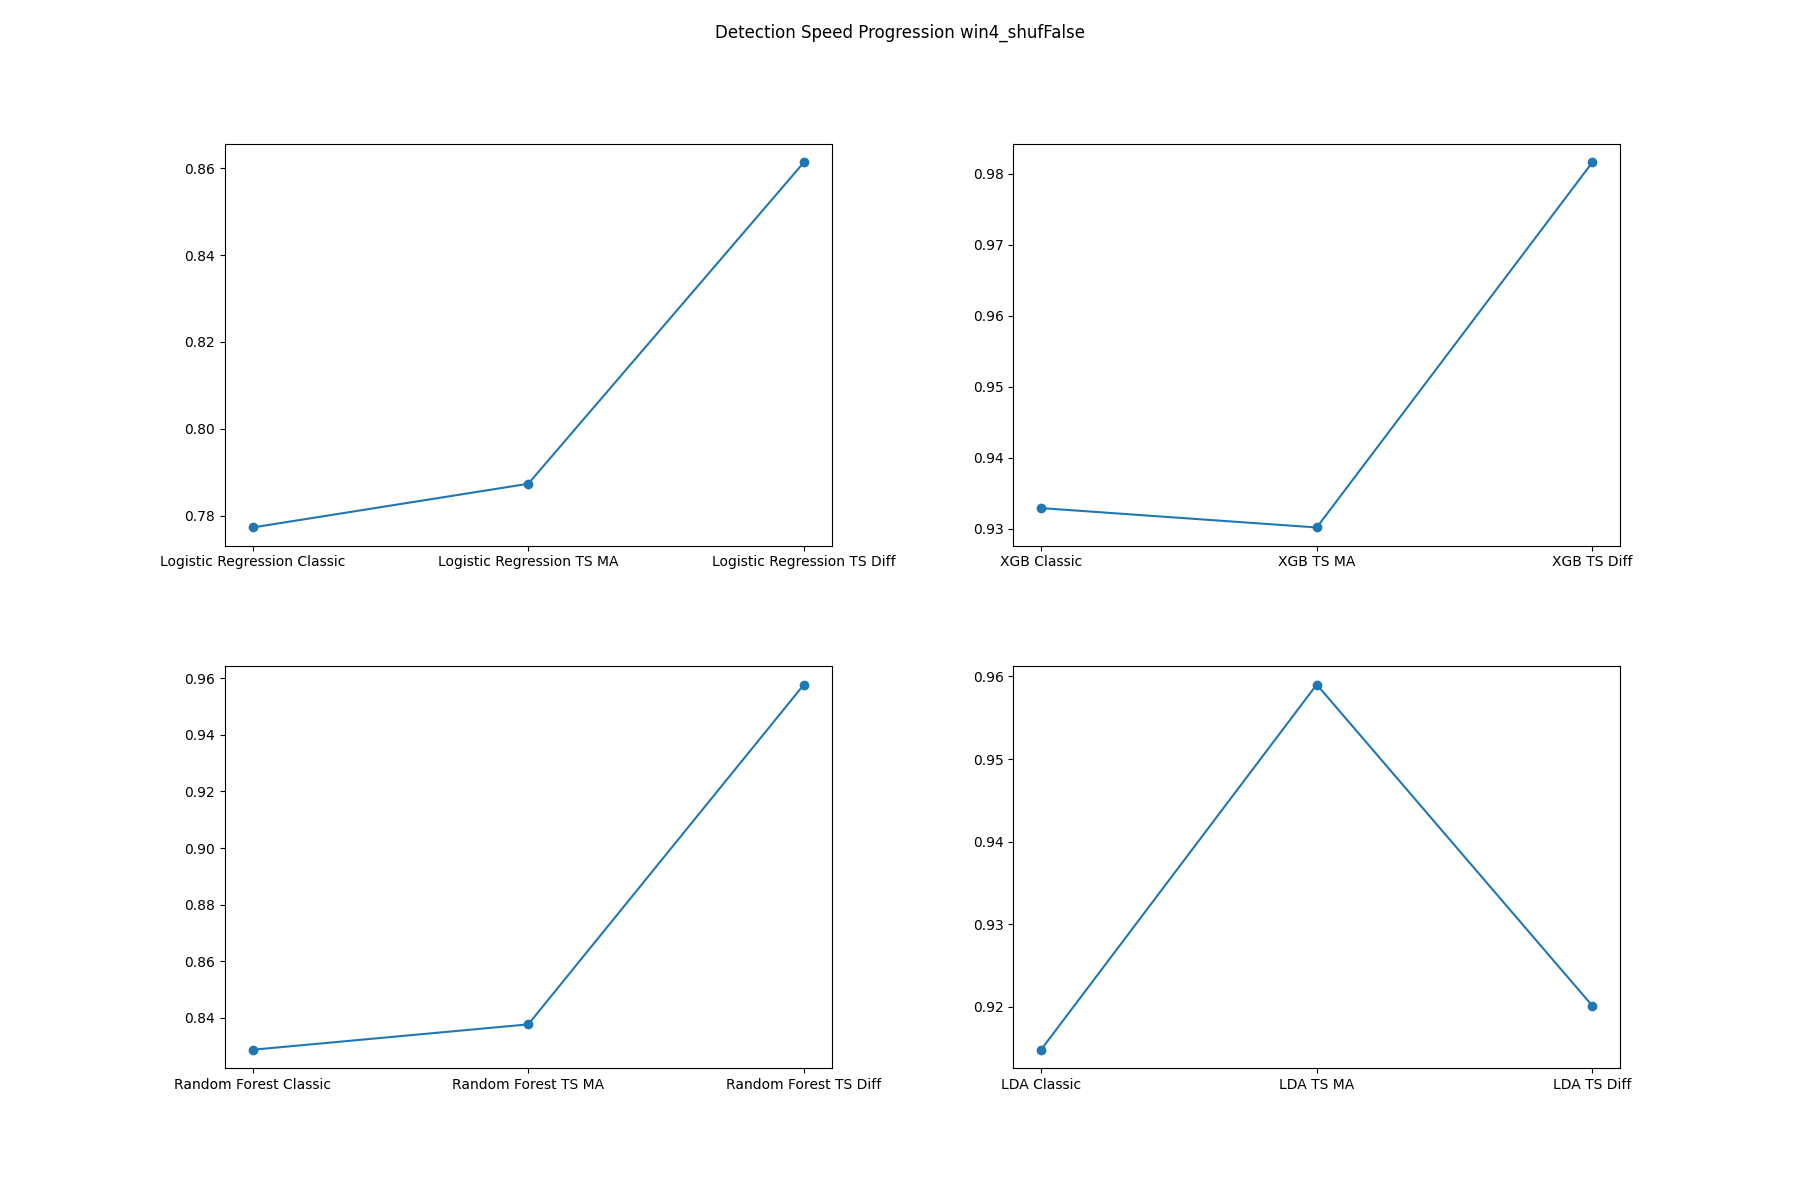
\includegraphics[width=0.94\linewidth]{Speed_Progression_win4_shufFalse.png}
    \caption{Progressione Speed Score window=4,shuffle=False}
    \label{fig:enter-label}
    \end{figure}

    \newpage
    \item \textit{\textbf{window = 3}, shuffle = False}:
    \begin{figure}[H]
    \centering
    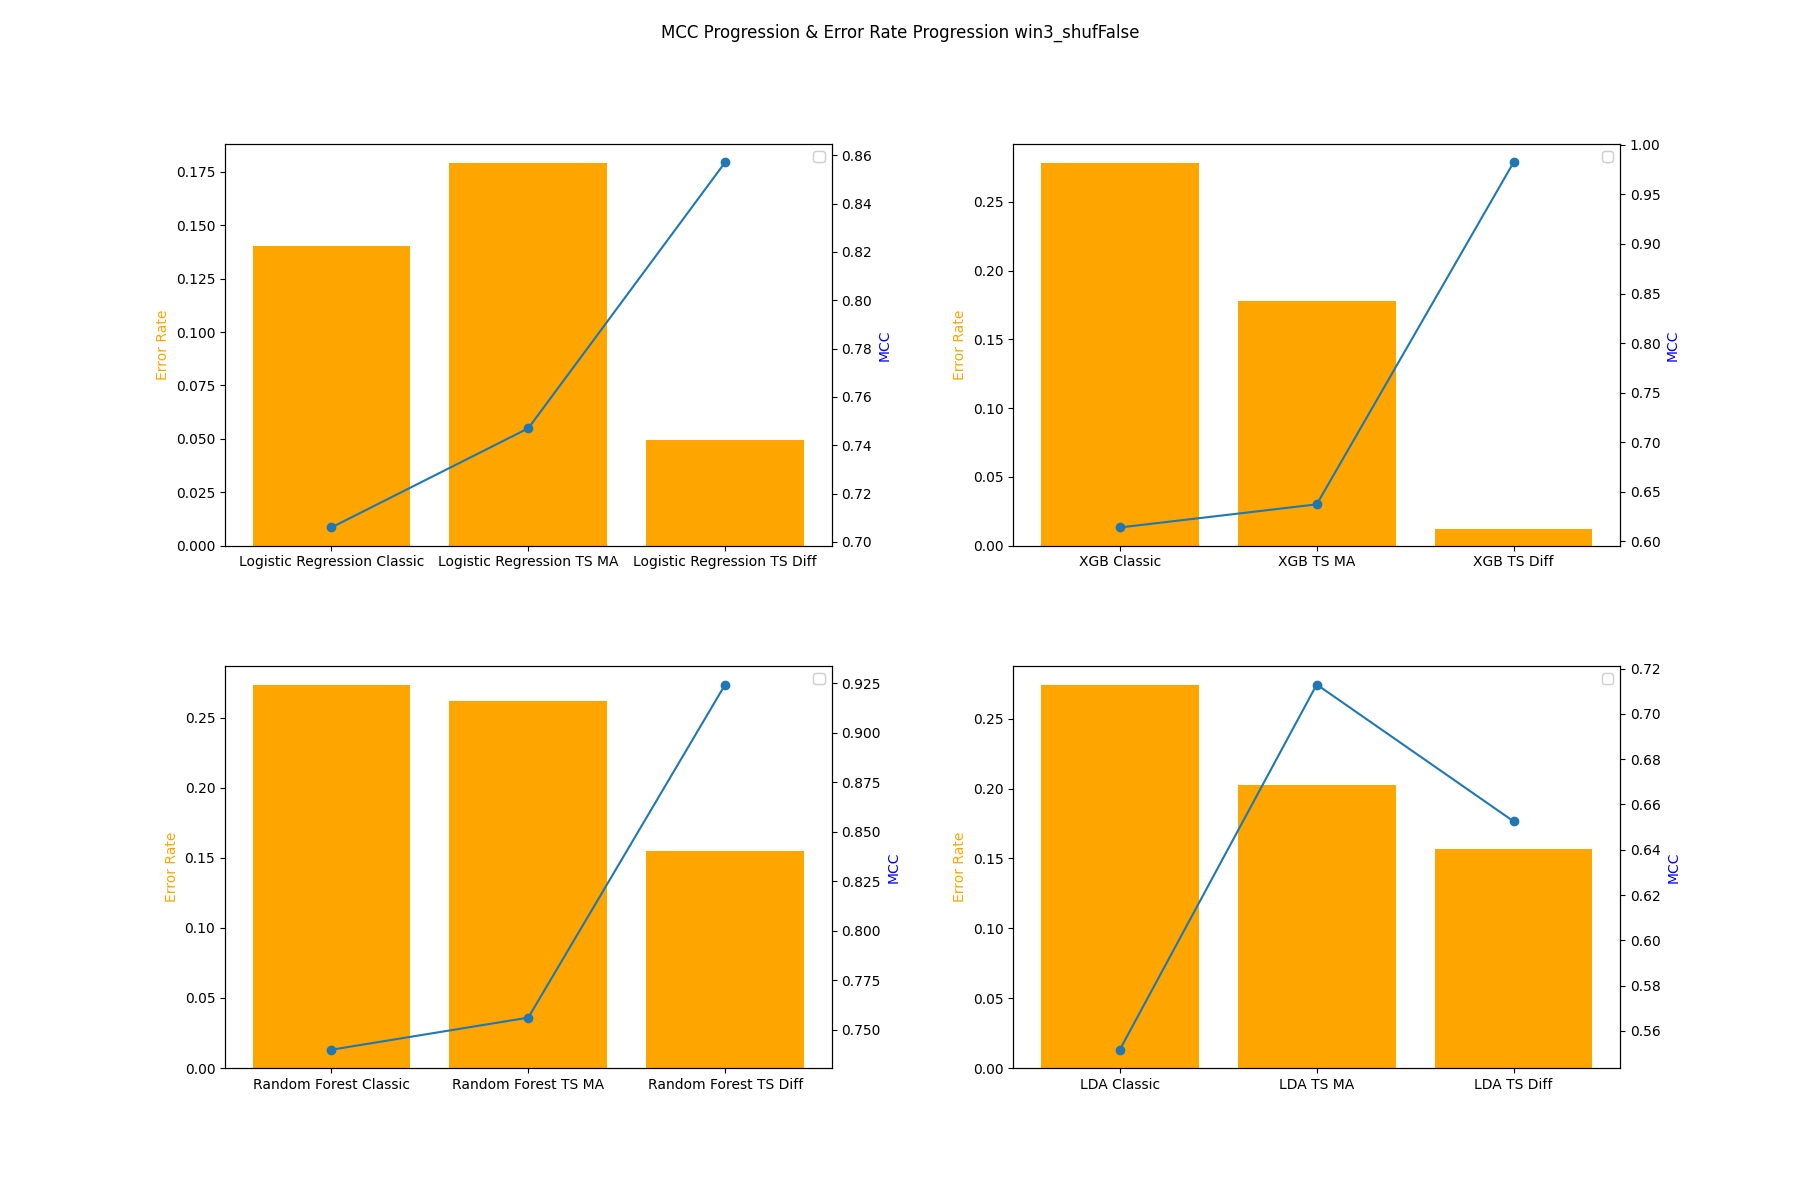
\includegraphics[width=0.94\linewidth]{MCC_Progression_win3_shufFalse.png}
    \caption{Progressione MCC ed Error Rate window=3,shuffle=False}
    \label{fig:enter-label}
    \end{figure}
    \begin{figure}[H]
    \centering
    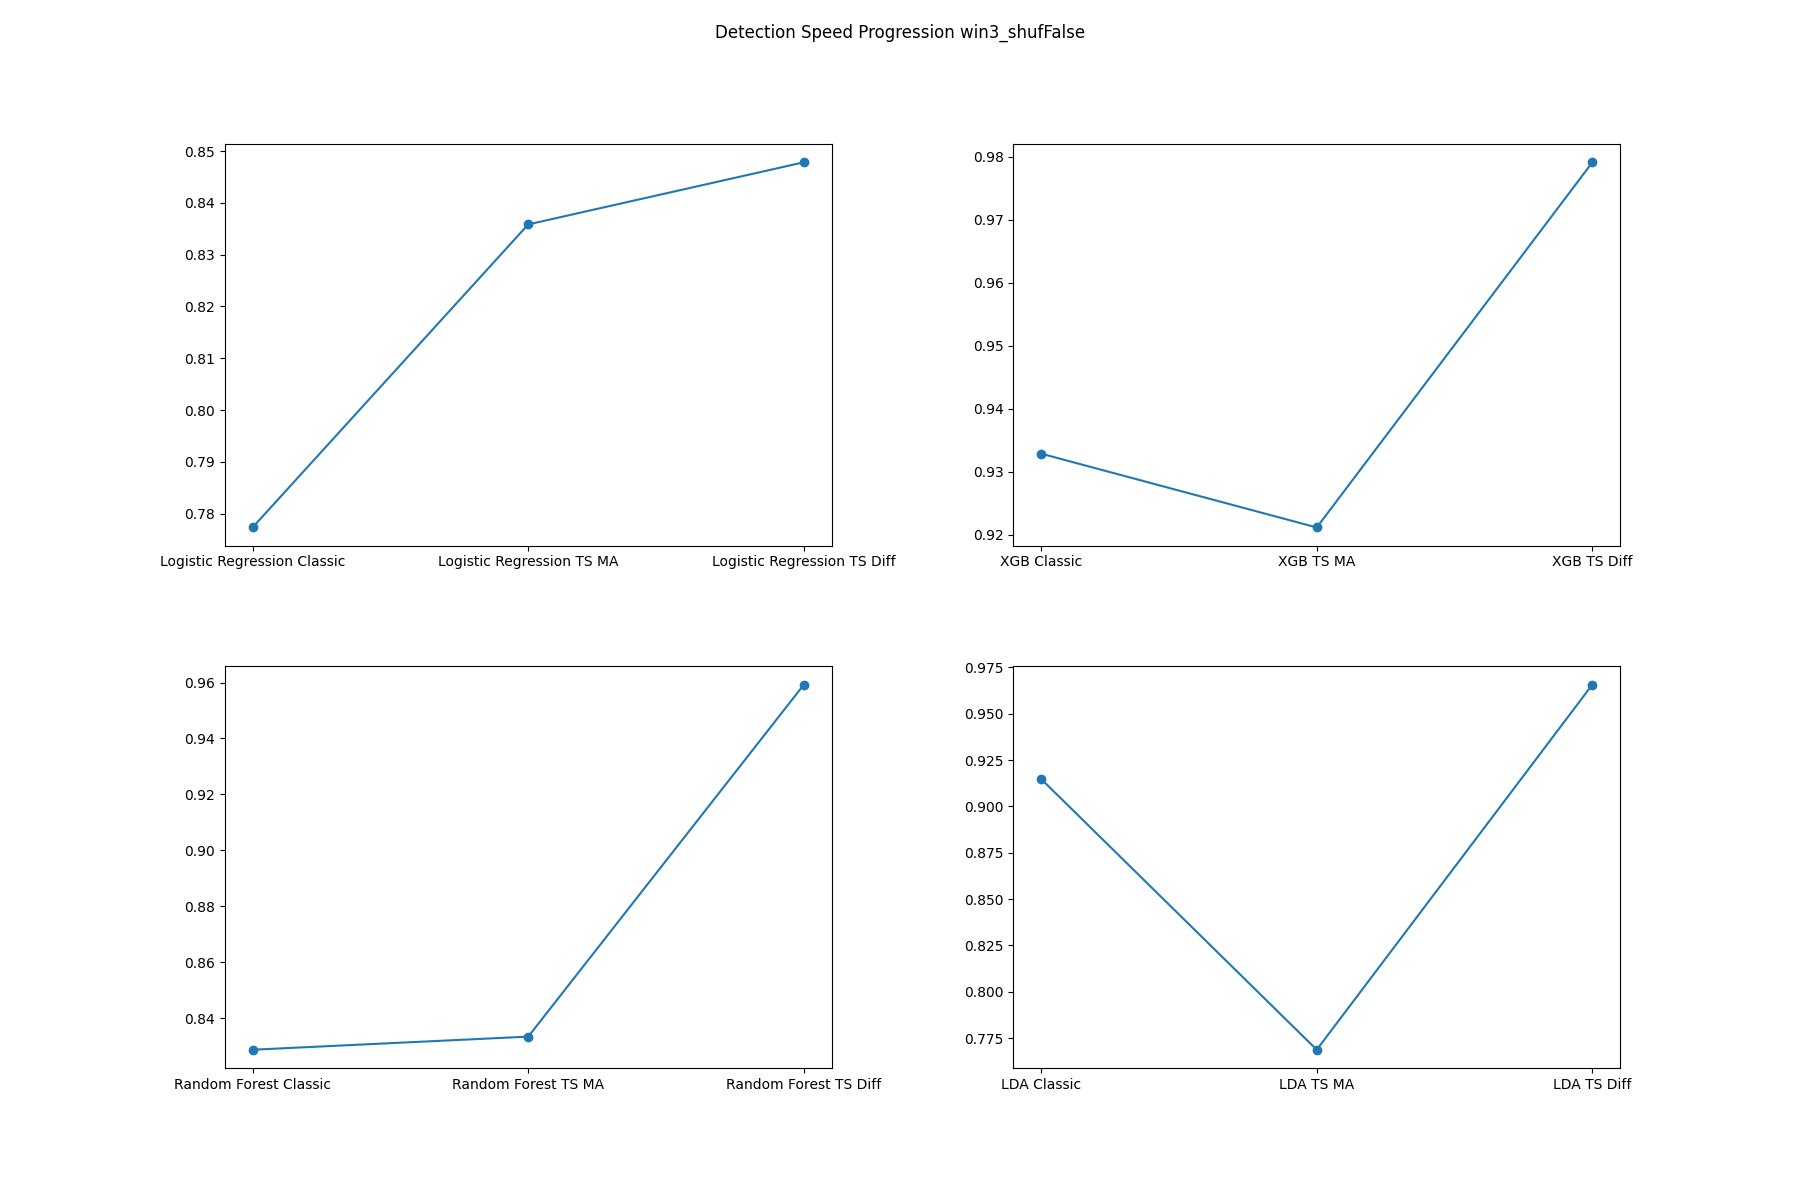
\includegraphics[width=0.94\linewidth]{Speed_Progression_win3_shufFalse.png}
    \caption{Progressione Speed Score window=3,shuffle=False}
    \label{fig:enter-label}
    \end{figure}

    \newpage
    \item \textit{\textbf{window = 2}, shuffle = False}:
    \begin{figure}[H]
    \centering
    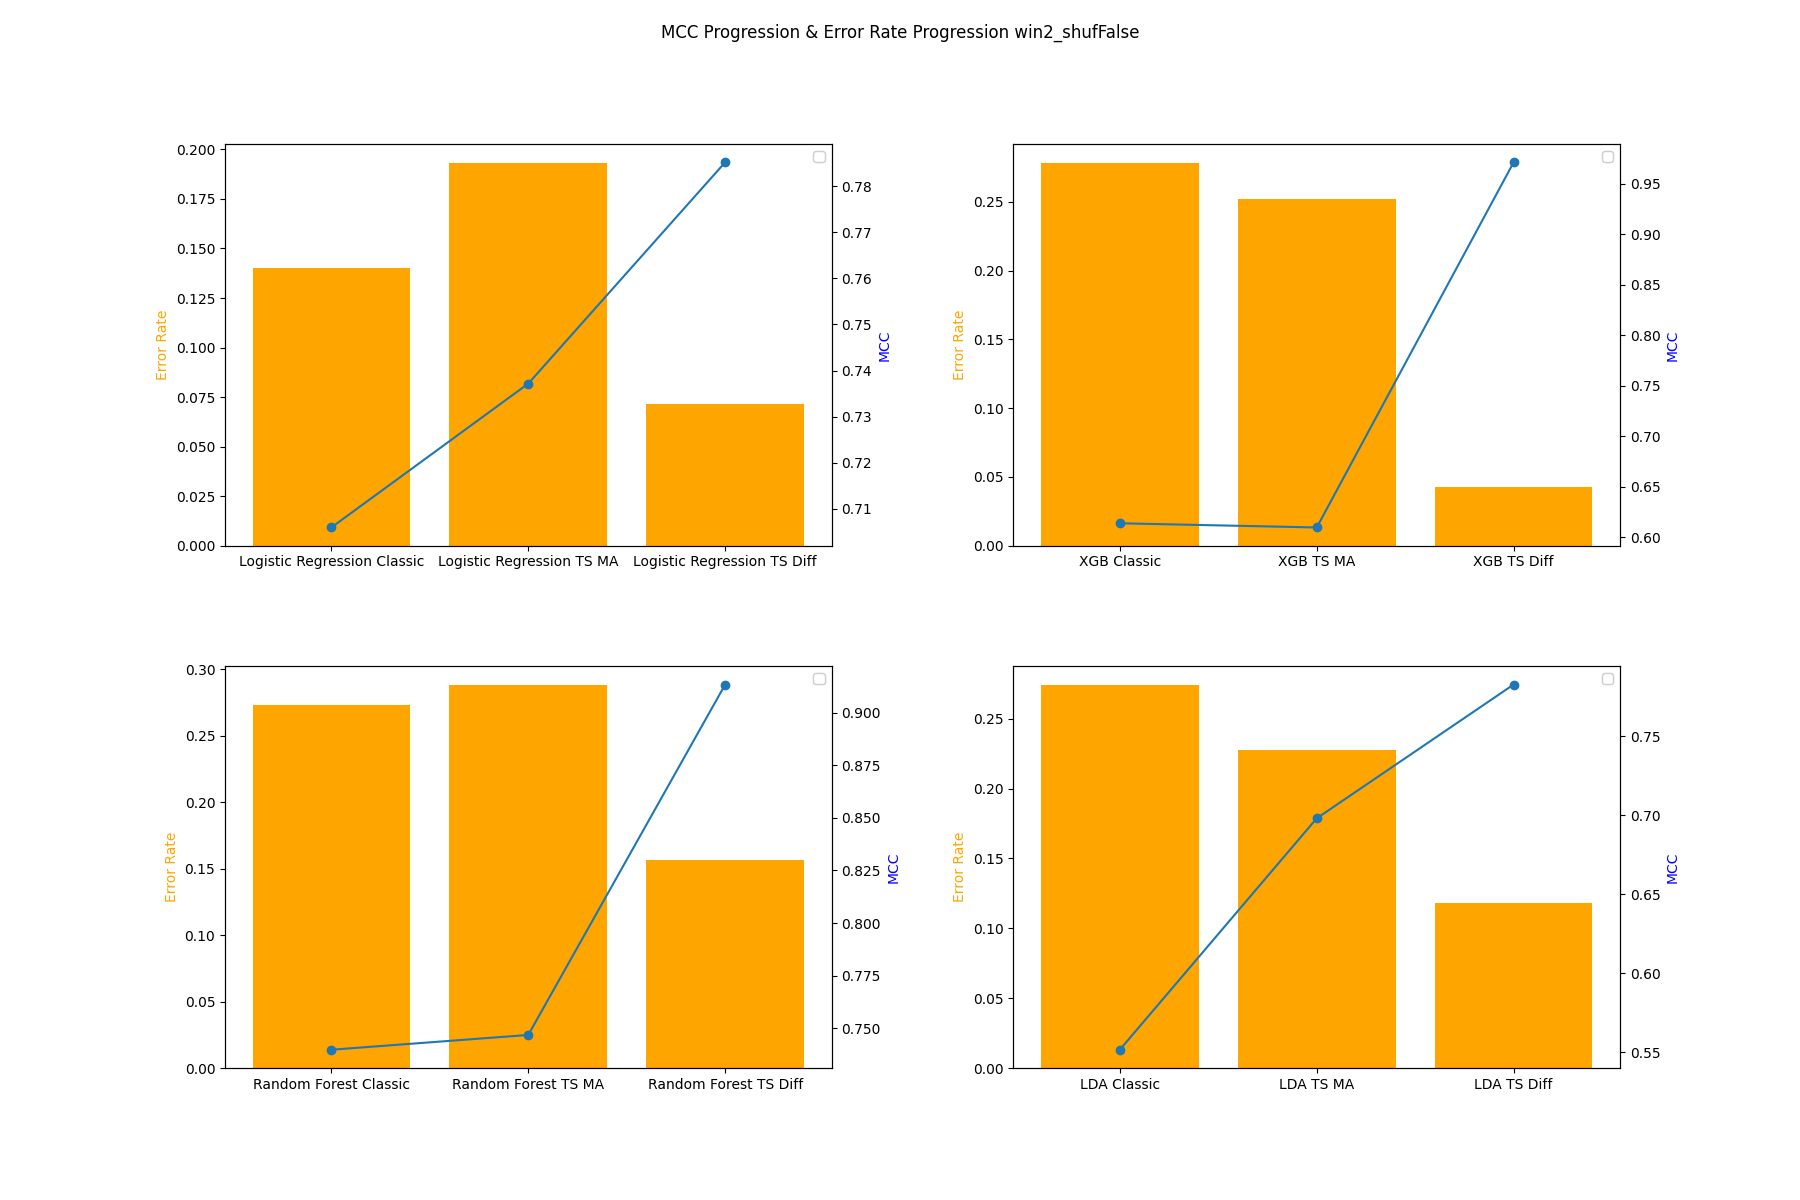
\includegraphics[width=0.94\linewidth]{MCC_Progression_win2_shufFalse.png}
    \caption{Progressione MCC ed Error Rate window=2,shuffle=False}
    \label{fig:enter-label}
    \end{figure}
    \begin{figure}[H]
    \centering
    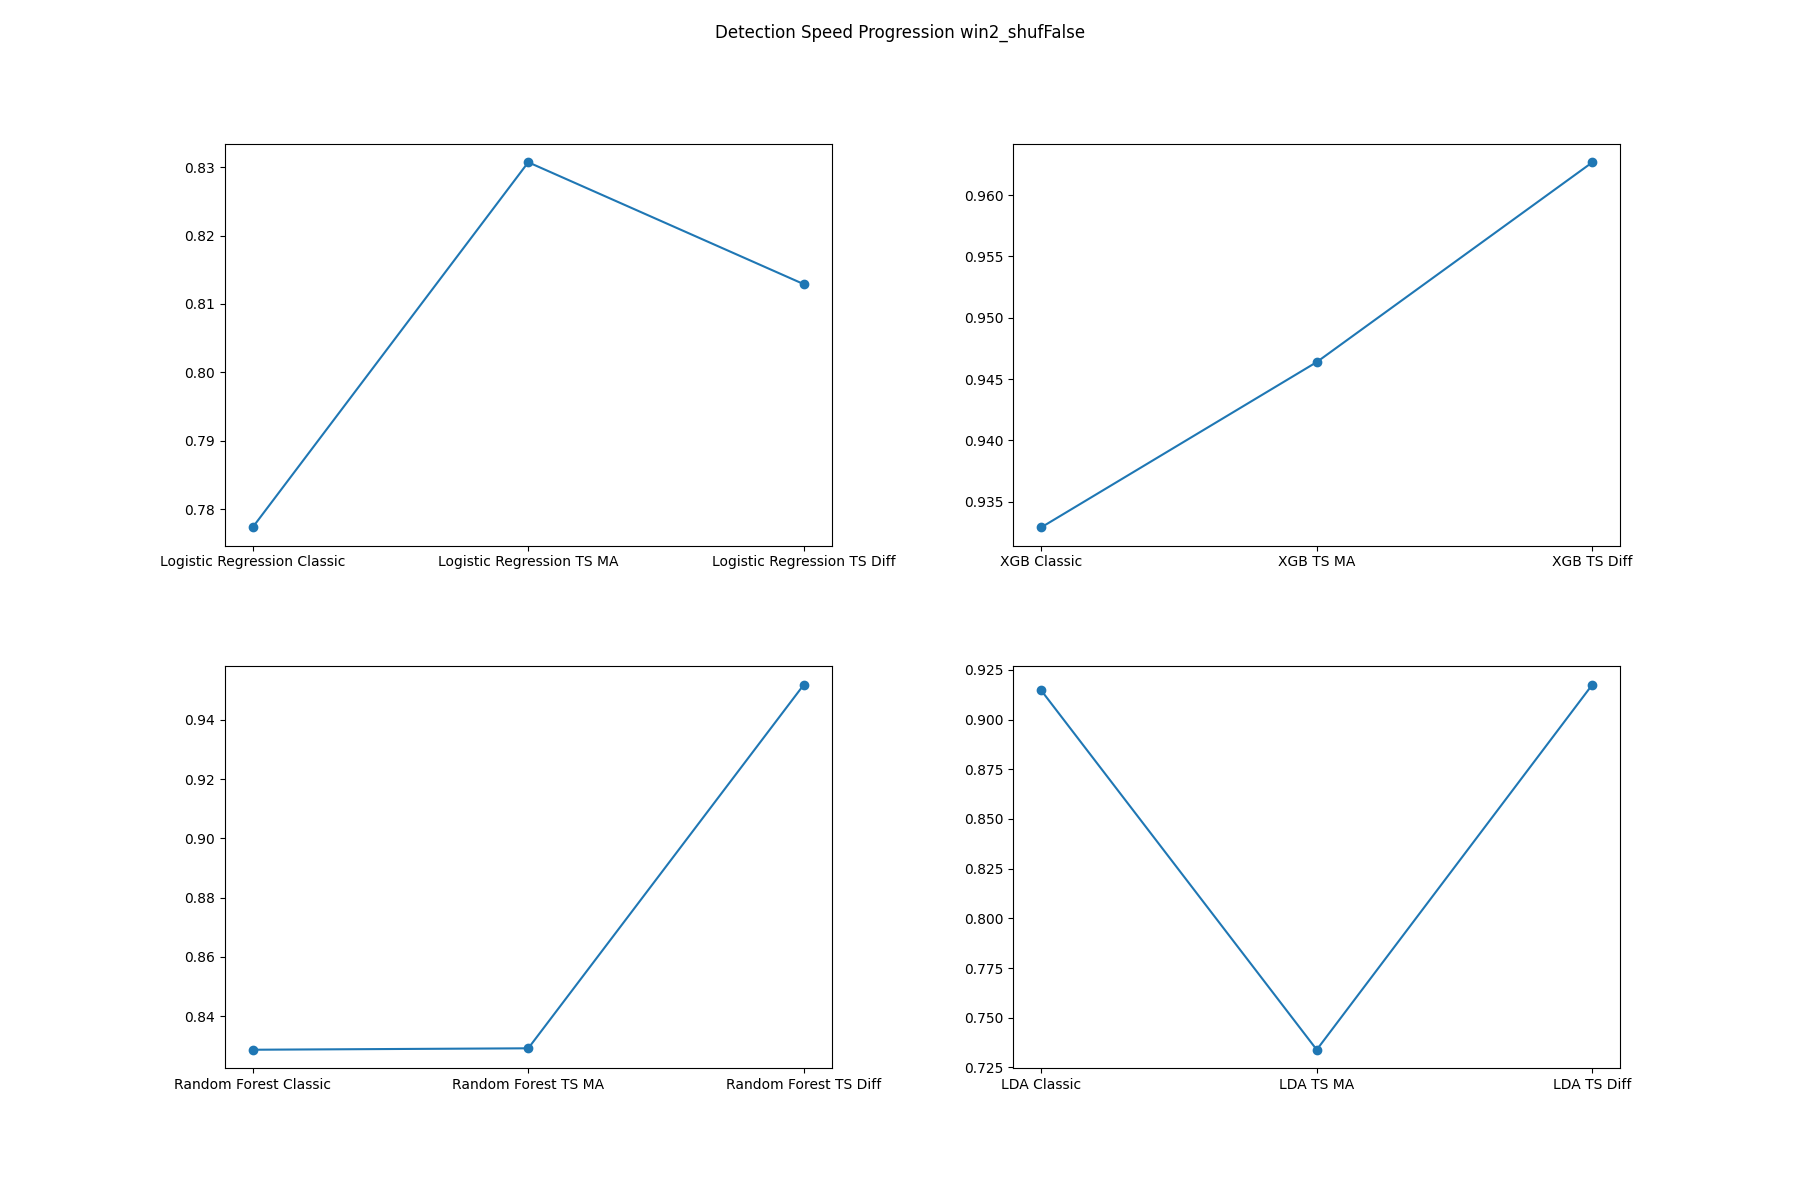
\includegraphics[width=0.94\linewidth]{Speed_Progression_win2_shufFalse.png}
    \caption{Progressione Speed Score window=2,shuffle=False}
    \label{fig:enter-label}
    \end{figure}
\end{itemize}

\newpage
I risultati ottenuti mostrano delle chiare tendenze:

\begin{itemize}

    \item Nell'87.5\% dei modelli (14 su 16) l'MCC \`e sempre crescente nel seguente ordine: approccio classico (\textit{classic}), approccio time series con media mobile (\textit{TS-MA}) e approccio time series con differenze (\textit{TS-Diff}). In particolare, l'ultimo approccio menzionato, \`e sempre il migliore in termini di MCC. In media un approccio time series migliora l'MCC, scalato in un intervallo $[0,1]$, di 0.24 con picchi di miglioramento che variano da 0.16 a 0.38. Quindi, dato il valore medio di MCC per l'approccio \textit{classic} di 0.65 e un'incremento medio di 0.24 con gli approcci time series, abbiamo un miglioramento delle performance in media del 37\% in termini di MCC. Si ha quindi un ottimo aumento dei valori di MCC, con un miglioramento medio della metrica principale di pi\`u di $\frac{1}{3}$ rispetto ai valori ottenuti con un approccio classico.

    \item Nel 62.5\% dei modelli (10 su 16) l'error rate segue la stessa tendenza dell'MCC, ovvero valori crescenti nell'ordine: \textit{classic, TS-MA, TS-Diff}. Nel restante 37,5\% dei modelli si ha un error rate maggiore con l'approccio \textit{TS-MA} rispetto all'approccio \textit{classic}. Per tutti i modelli, invece, vale sempre che l'error rate minore \`e dato dall'approccio \textit{TS-Diff}. Il miglioramento medio di error rate da uno dei 2 approcci, \textit{classic} o \textit{TS-MA}, a un approccio \textit{TS-Diff} \`e di 0.16 con estremi di 0.11 e 0.27, ricordando che l'error rate \`e compreso in un intervallo $[0,1]$. Quindi, considerando per ogni modello l'error rate pi\`u alto tra approccio \textit{classic} e \textit{TS-MA}, passare ad un approccio \textit{TS-Diff} porta a un miglioramento delle performance in termini di error rate del 64\%, partendo da un error rate medio di 0.25 e avendo una decrescita media di 0.16. In conclusione, passare ad un approccio \textit{TS-Diff} porta a una significativa riduzione dell'error rate, che viene pi\`u che dimezzato.





    \item Per quanto riguarda lo speed score non c'\`e una chiara tendenza: la tendenza che si ha per l'MCC vale per lo speed score solo nel 50\% dei modelli (8 su 16). In particolare, per quanto riguarda questa metrica, la tendenza varia da algoritmo a algoritmo. Random Forest, ad esempio, segue sempre per ogni finestra temporale la tendenza prevalente per l'MCC. Anche Logistic Regression segue la stessa tendenza, a parte per la finestra temporale con \textit{window = 2} dove si ha in ordine crescente: approccio \textit{classic, TS-Diff, TS-MA}. Per XGBoost, invece, la tendenza in ordine crescente \`e la seguente: approccio \textit{TS-MA, classic, TS-Diff} a parte per i modelli con \textit{window = 2} dove la tendenza corrisponde a quella prevalente per l'MCC. Infine, per l'algoritmo LDA, nei modelli addestrati su finestra temporale con \textit{window = 4} e {window = 5} si hanno valori crescenti di speed score nel seguente ordine: approccio \textit{classic, TS-Diff, TS-MA}. Mentre per i modelli con \textit{window = 3} e {window = 2} si ha: approccio \textit{TS-MA, classic, TS-Diff}. Questa metrica \`e sicuramente la meno robusta tra tutte le metriche prese in considerazione perch\'e considera solo la velocit\`a con cui l'anomalia viene rilevata senza prendere in considerazione l'accuratezza della previsione stessa, non essendo presente nella sua formula alcuna forma di penalizzazione in caso di previsione sbagliata. Tale metrica \`e da considerarsi come benchmark secondario da affiancare a una metrica robusta di riferimento come l'MCC.
    
\end{itemize}


\section{MCC dataset my-all3}
In questa sezione si sono analizzati i risultati che hanno ottenuto i modelli, in termini di MCC, usando come set di test il dataset \textit{my-all3}. Nella prossima pagina sono presenti i grafici comparativi tra la progressione dell'MCC sul test set di \textit{unifi-filtered} e sul dataset \textit{my-all3}.


\begin{itemize}
    \newpage
    \item \textit{\textbf{window = 5}, shuffle = False}:
    \begin{figure}[H]
    \centering
    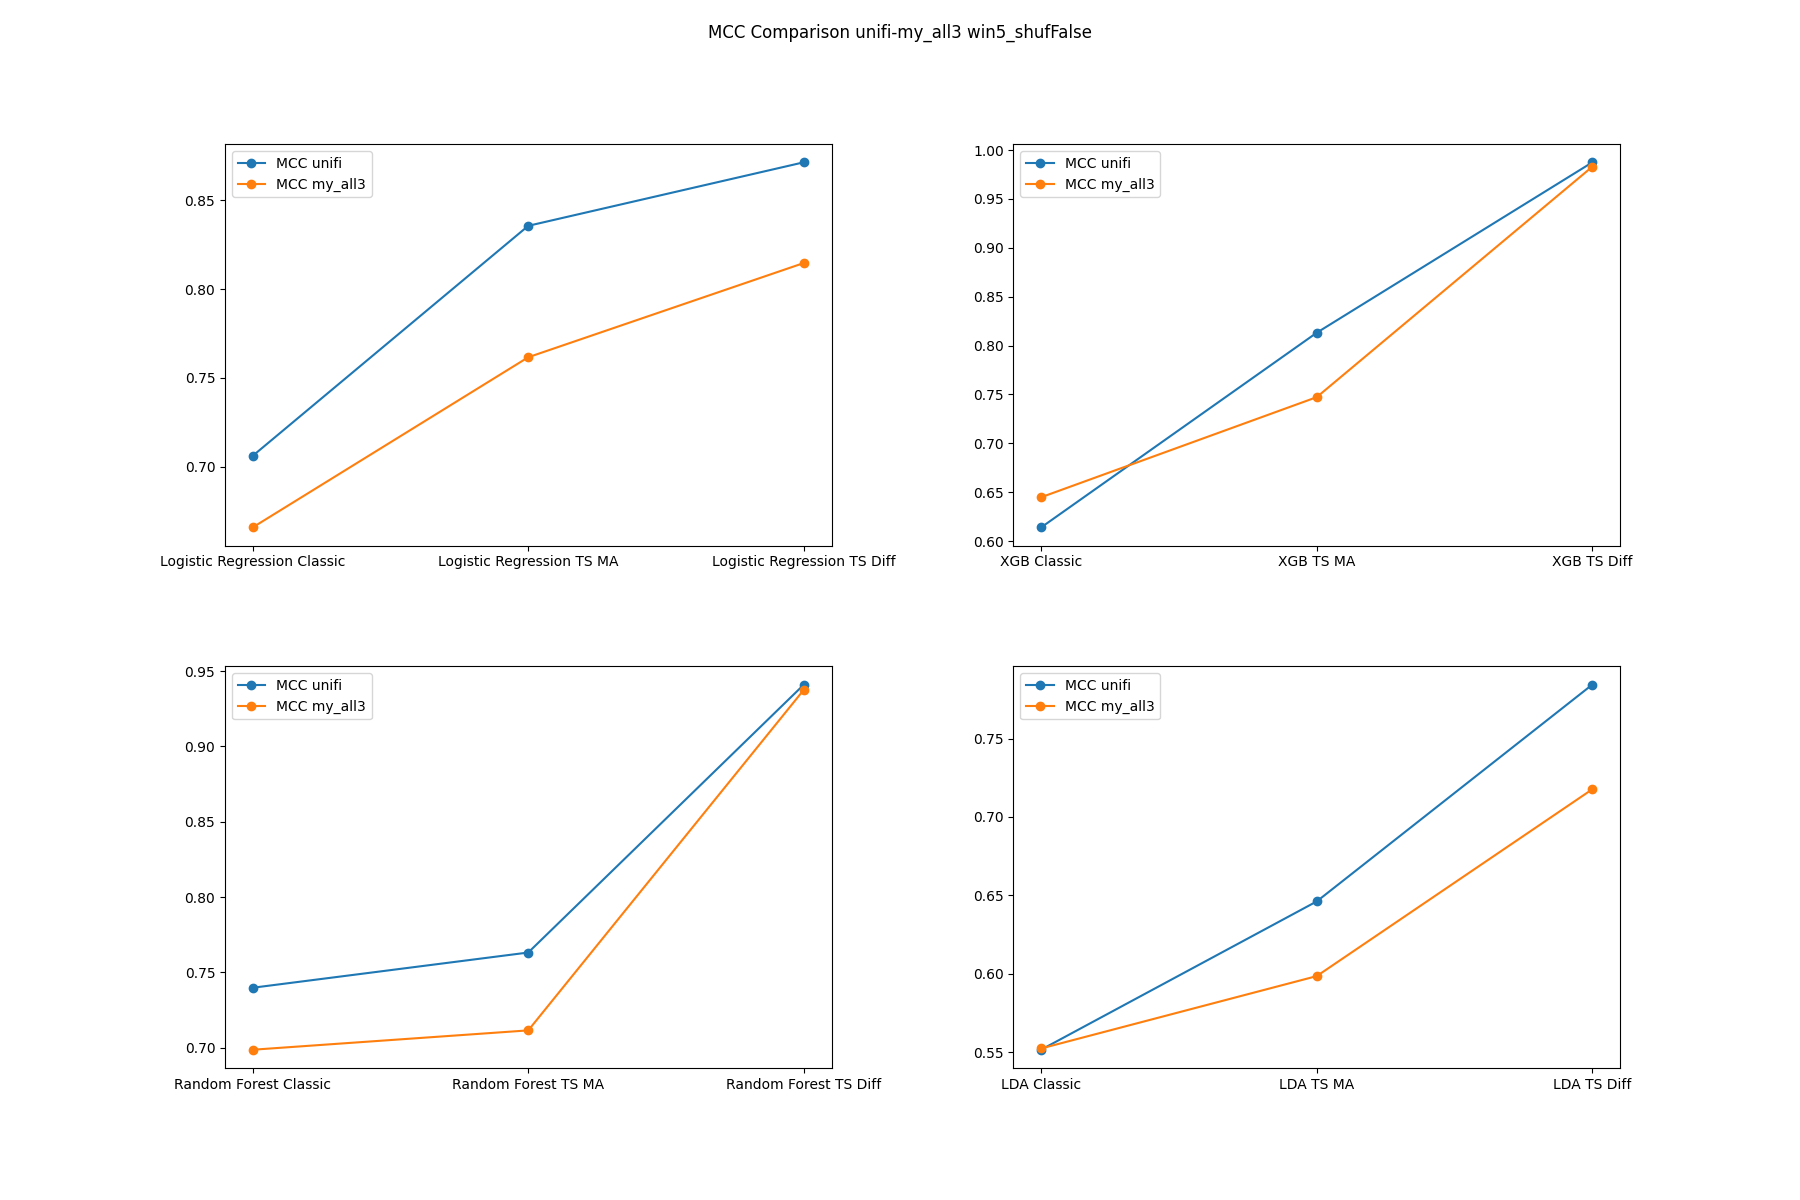
\includegraphics[width=0.94\linewidth]{MCC Comparison Uni-All3 win5_shufFalse.png}
    \caption{Comparazione MCC unifi e my-all3 window=5,shuffle=False}
    \label{fig:enter-label}
    \end{figure}

    \item \textit{\textbf{window = 4}, shuffle = False}:
    \begin{figure}[H]
    \centering
    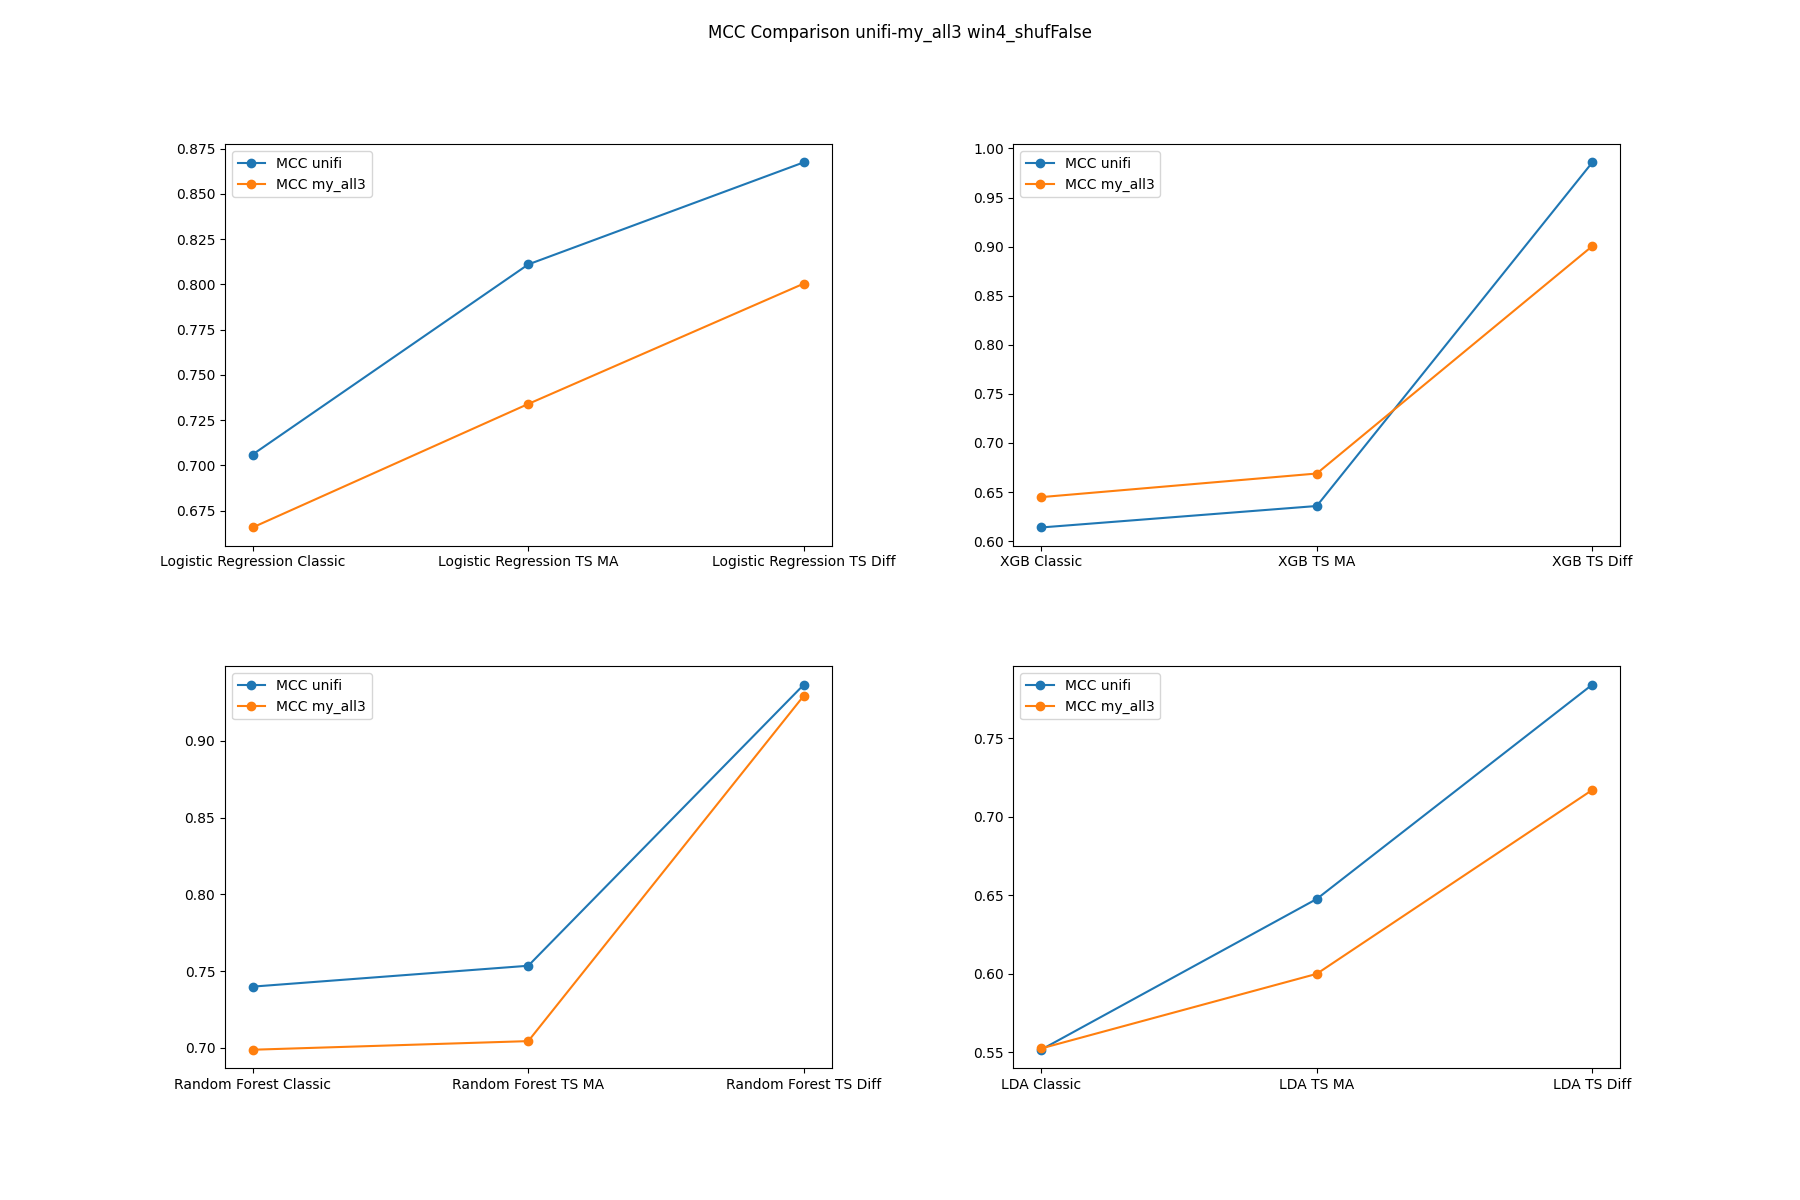
\includegraphics[width=0.94\linewidth]{MCC Comparison Uni-All3 win4_shufFalse.png}
    \caption{Comparazione MCC unifi e my-all3 window=4,shuffle=False}
    \label{fig:enter-label}
    \end{figure}

    \newpage
    \item \textit{\textbf{window = 3}, shuffle = False}:
    \begin{figure}[H]
    \centering
    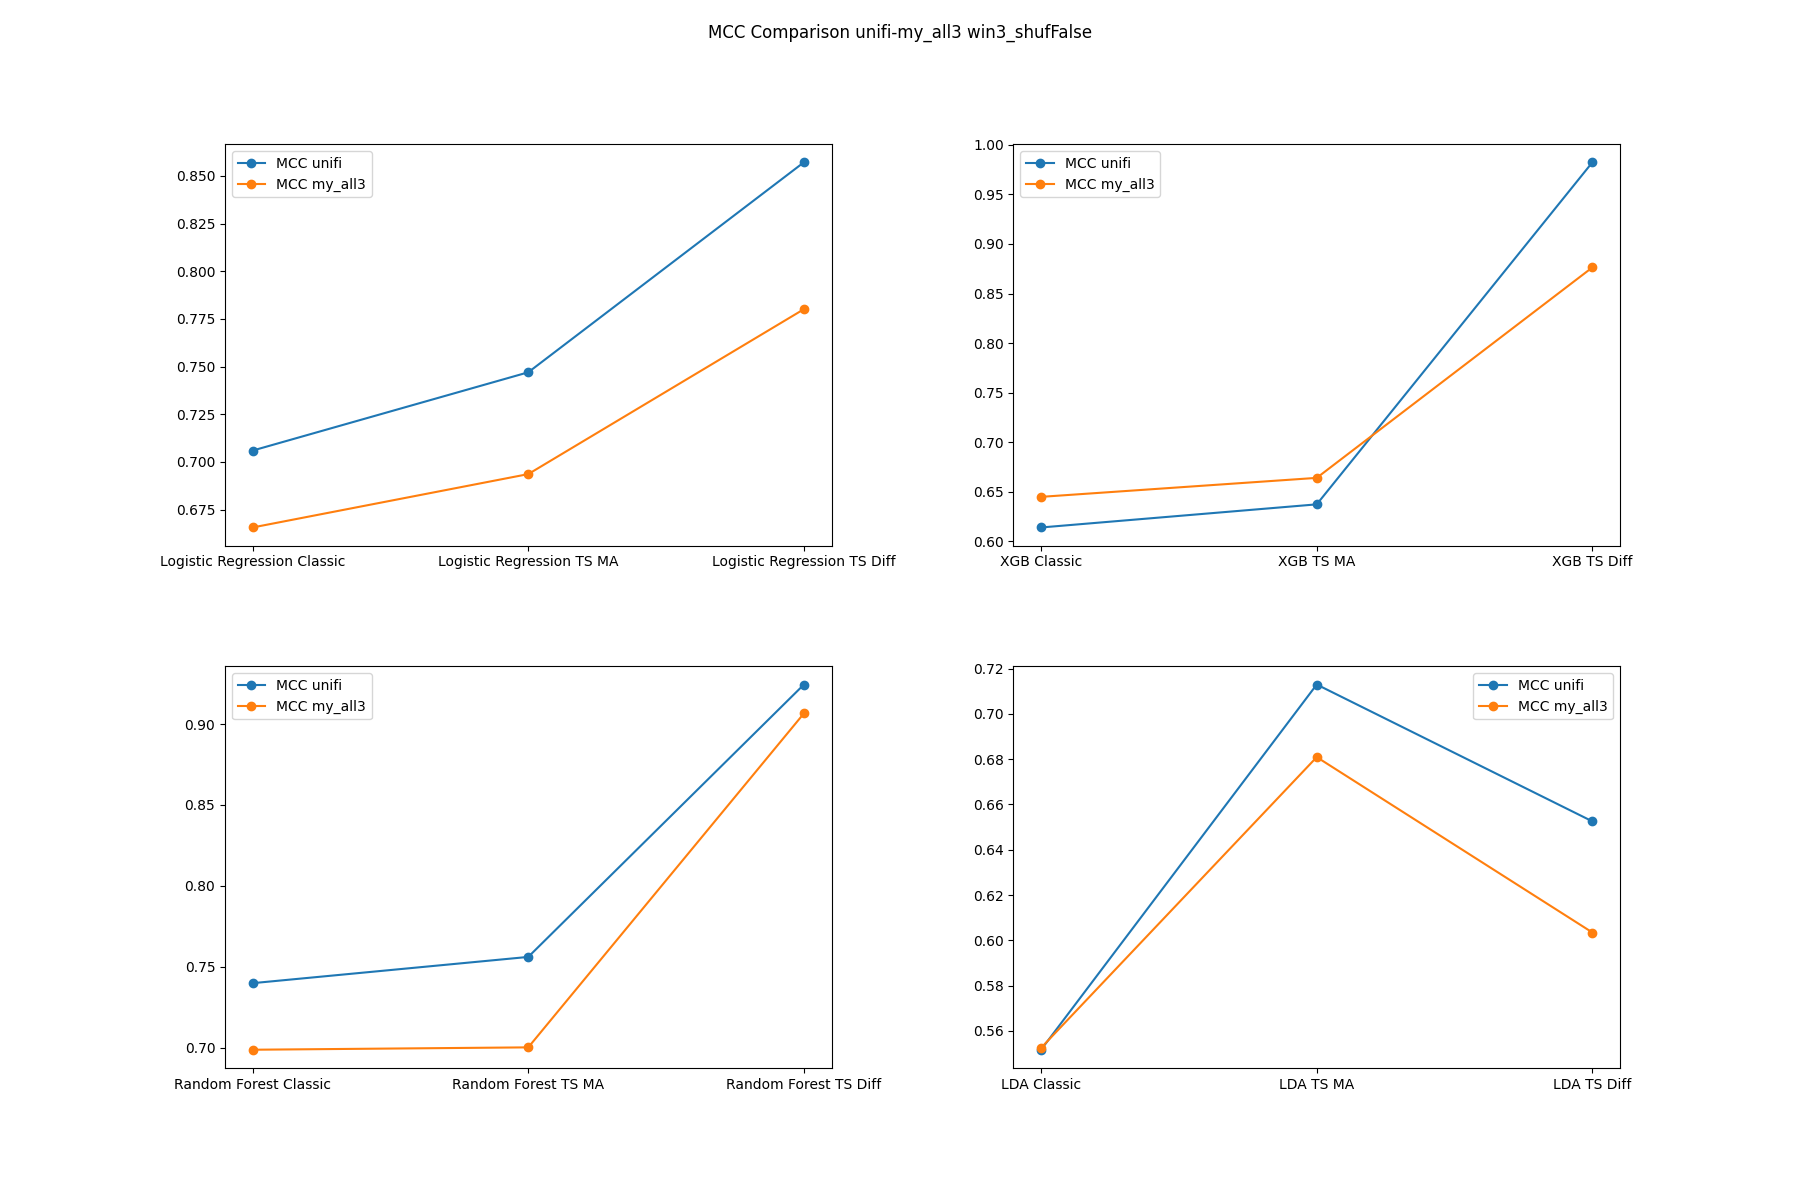
\includegraphics[width=0.94\linewidth]{MCC Comparison Uni-All3 win3_shufFalse.png}
    \caption{Comparazione MCC unifi e my-all3 window=3,shuffle=False}
    \label{fig:enter-label}
    \end{figure}

    \item \textit{\textbf{window = 2}, shuffle = False}:
    \begin{figure}[H]
    \centering
    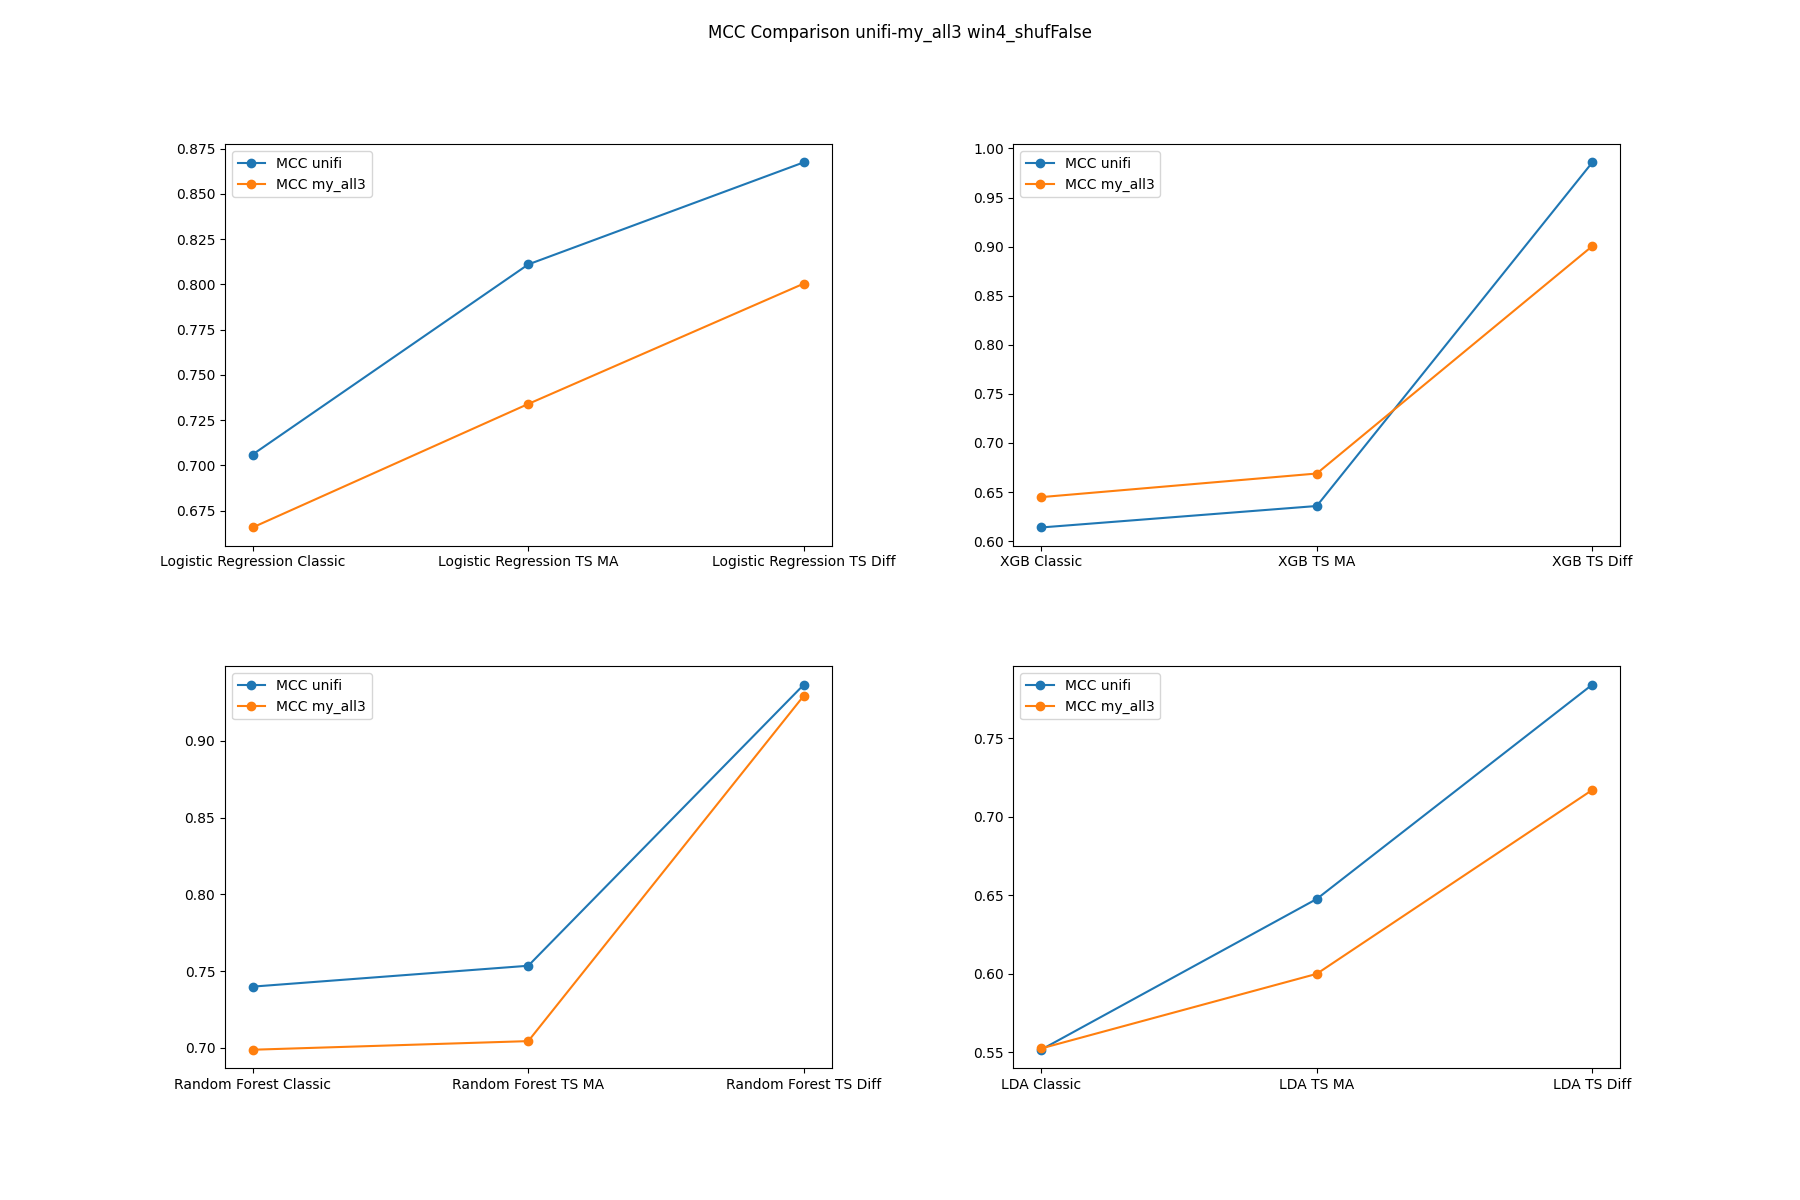
\includegraphics[width=0.94\linewidth]{MCC Comparison Uni-All3 win4_shufFalse.png}
    \caption{Comparazione MCC unifi e my-all3 window=2,shuffle=False}
    \label{fig:enter-label}
    \end{figure}
\end{itemize}

\newpage
Come si pu\`o notare dai risultati ottenuti per la maggior parte dei modelli, come ci si pu\`o aspettare, le performance sono migliori sul test set di \textit{unifi-filtered}, perch\'e i modelli sono stati addestrati su questa istanza del problema. In altri casi, si hanno performance leggermente migliori sul dataset \textit{my-all3}. In generale si pu\`o dire che i modelli hanno generalizzato discretamente, non essendoci grandi differenze di MCC tra i due dataset. Sicuramente possiamo notare come la tendenza nella progressione dell'MCC sia sempre omogenea tra test set di \textit{unifi-filtered} e \textit{my-all3}.

\section{Progressione MCC al variare della finestra temporale}
Un altro aspetto su cui si \`e posta l'attenzione \`e la variazione dell'MCC negli approcci time series al variare della finestra temporale. \`E un aspetto interessante da analizzare perch\'e ci consente di trovare qual \`e la finestra temporale ottimale da utlizzare, a seconda delle esigenze. Una finestra temporale pi\`u ampia fornisce sicuramente al modello pi\`u informazioni da cui apprendere, ma al tempo stesso comporta una moltiplicazione non indifferente delle features nel dataset. \`E stato quindi rappresentato il grafico della progressione dell'MCC per gli approcci time series al variare della finestra temporale, per tutti i tipi di modelli.

\begin{figure}[H]
    \centering
    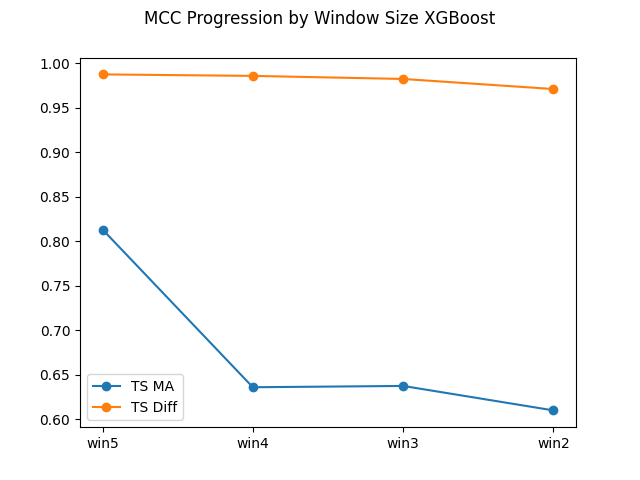
\includegraphics[width=0.78\linewidth]{MCC_Progression_by_Window_Size_XGBoost.png}
    \caption{Progressione MCC XGBoost in base alla finestra temporale}
    \label{fig:enter-label}
\end{figure}

\begin{figure}[H]
    \centering
    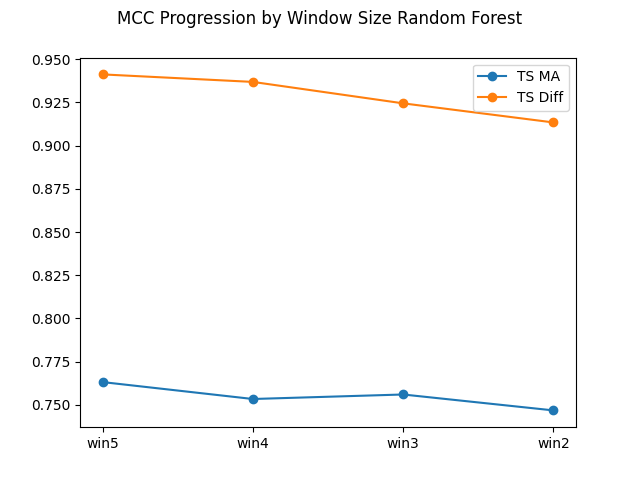
\includegraphics[width=0.78\linewidth]{MCC_Progression_by_Window_Size_Random Forest.png}
    \caption{Progressione MCC Random Forest in base alla finestra temporale}
    \label{fig:enter-label}
\end{figure}

\vspace{3cm}

\begin{figure}[H]
    \centering
    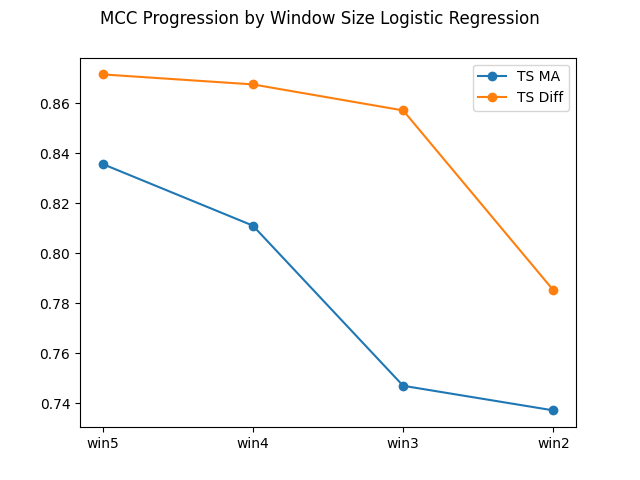
\includegraphics[width=0.78\linewidth]{MCC_Progression_by_Window_Size_Logistic Regression.png}
    \caption{Progressione MCC Logistic Regression in base alla finestra temporale}
    \label{fig:enter-label}
\end{figure}

\begin{figure}[H]
    \centering
    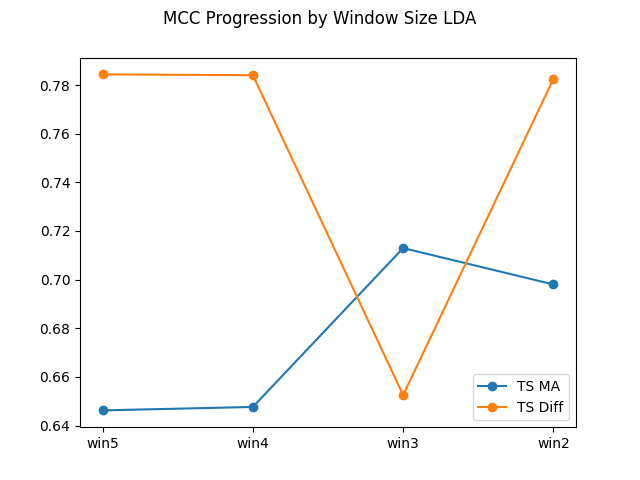
\includegraphics[width=0.78\linewidth]{MCC_Progression_by_Window_Size_LDA.png}
    \caption{Progressione MCC LDA in base alla finestra temporale}
    \label{fig:enter-label}
\end{figure}

\vspace{0.5 cm}

Dalle progressioni vediamo come le tendenze cambino da algoritmo a algoritmo. In generale, comunque, l'MCC a parte per poche eccezioni, diminuisce al diminuire dell'ampiezza della finestra temporale, avendo il modello meno dati a disposizione durante l'apprendimento.
\newpage


\section{Confronto shuffle True/False}
Nella presente sezione si sono volute analizzare le performance e le differenze dei modelli addestrati con il parametro \textit{shuffle = True}. Possiamo osservare nei grafici riportati qui sotto la progressione dell'MCC nei modelli addestrati su una finestra temporale \textit{window = 5} con \textit{shuffle = True} e \textit{shuffle = False}.

\begin{figure}[H]
    \centering
    \subfloat[Shuffle = True]{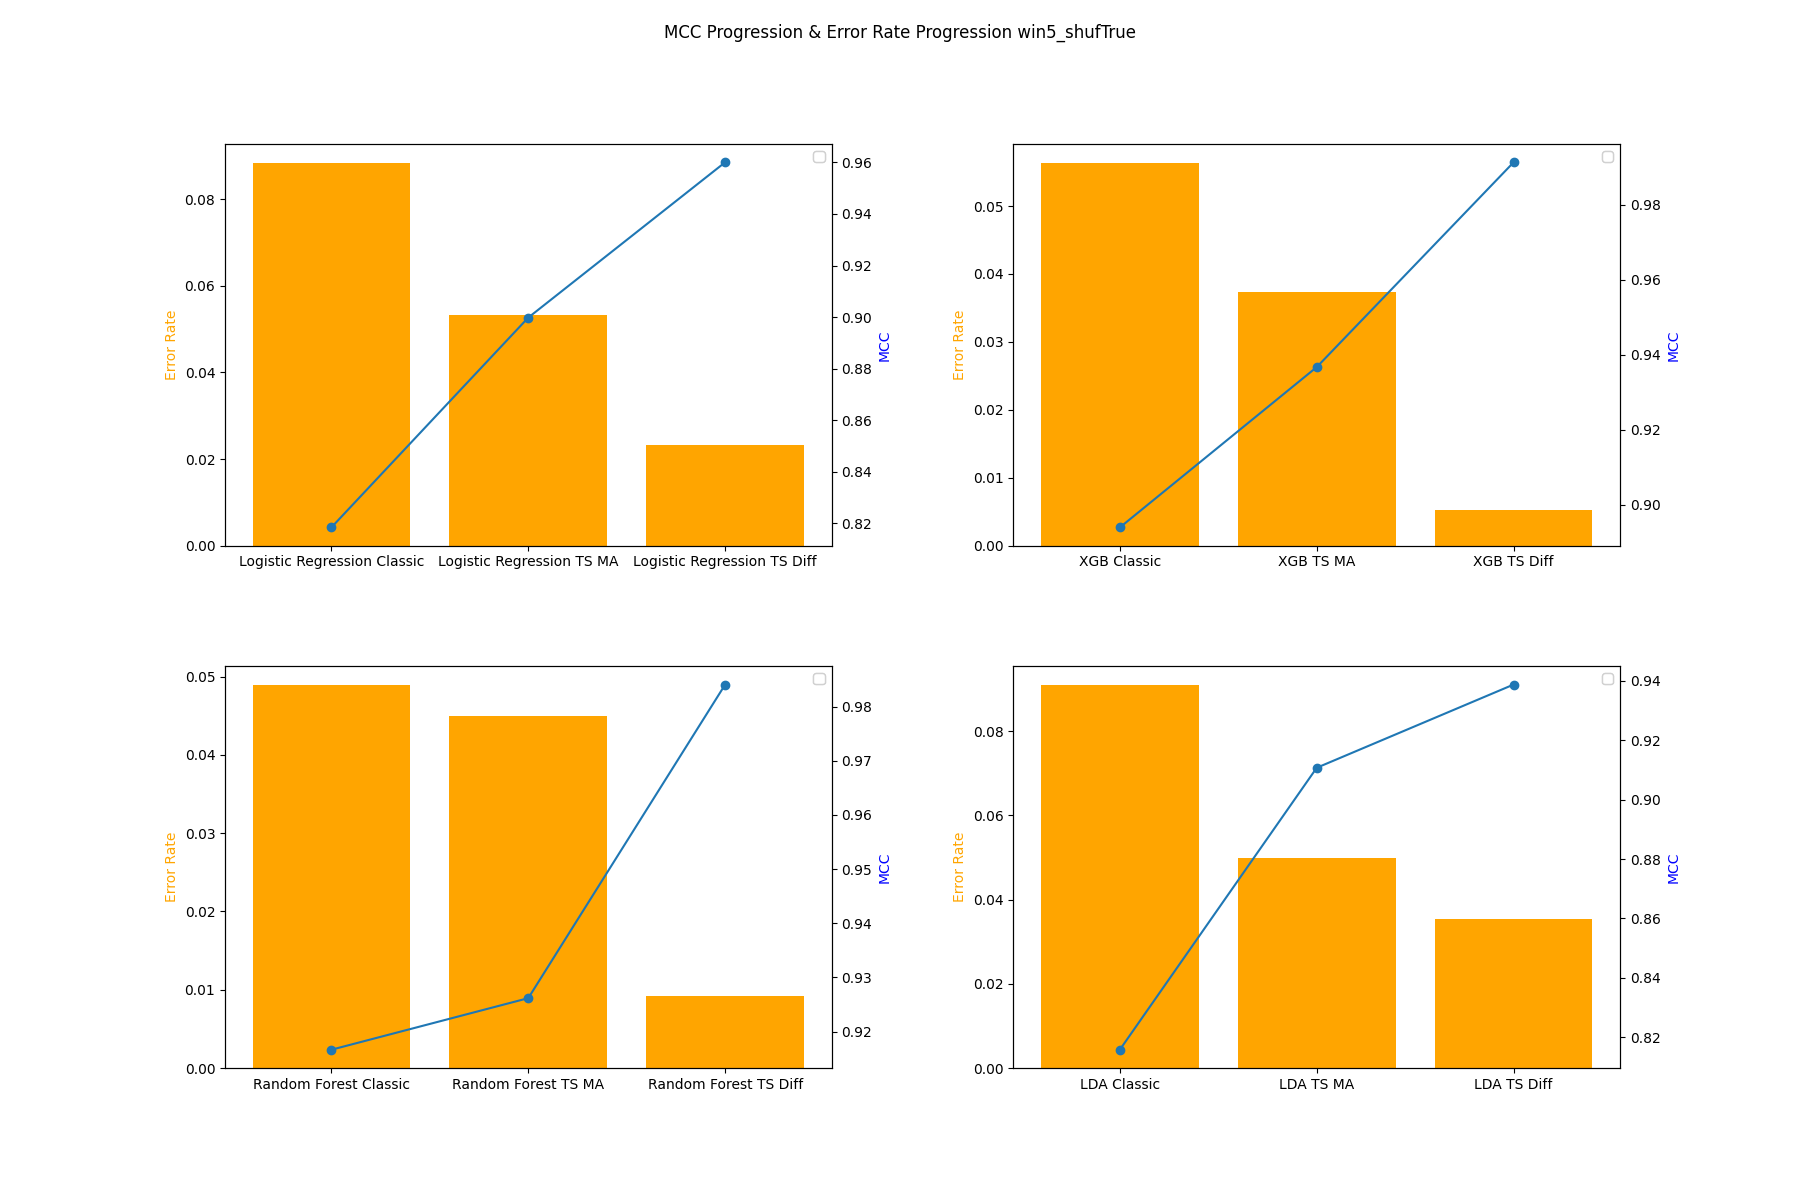
\includegraphics[width=0.8\textwidth]{MCC_Progression_win5_shufTrue.png}}
    \hfill
    \subfloat[Shuffle = False]{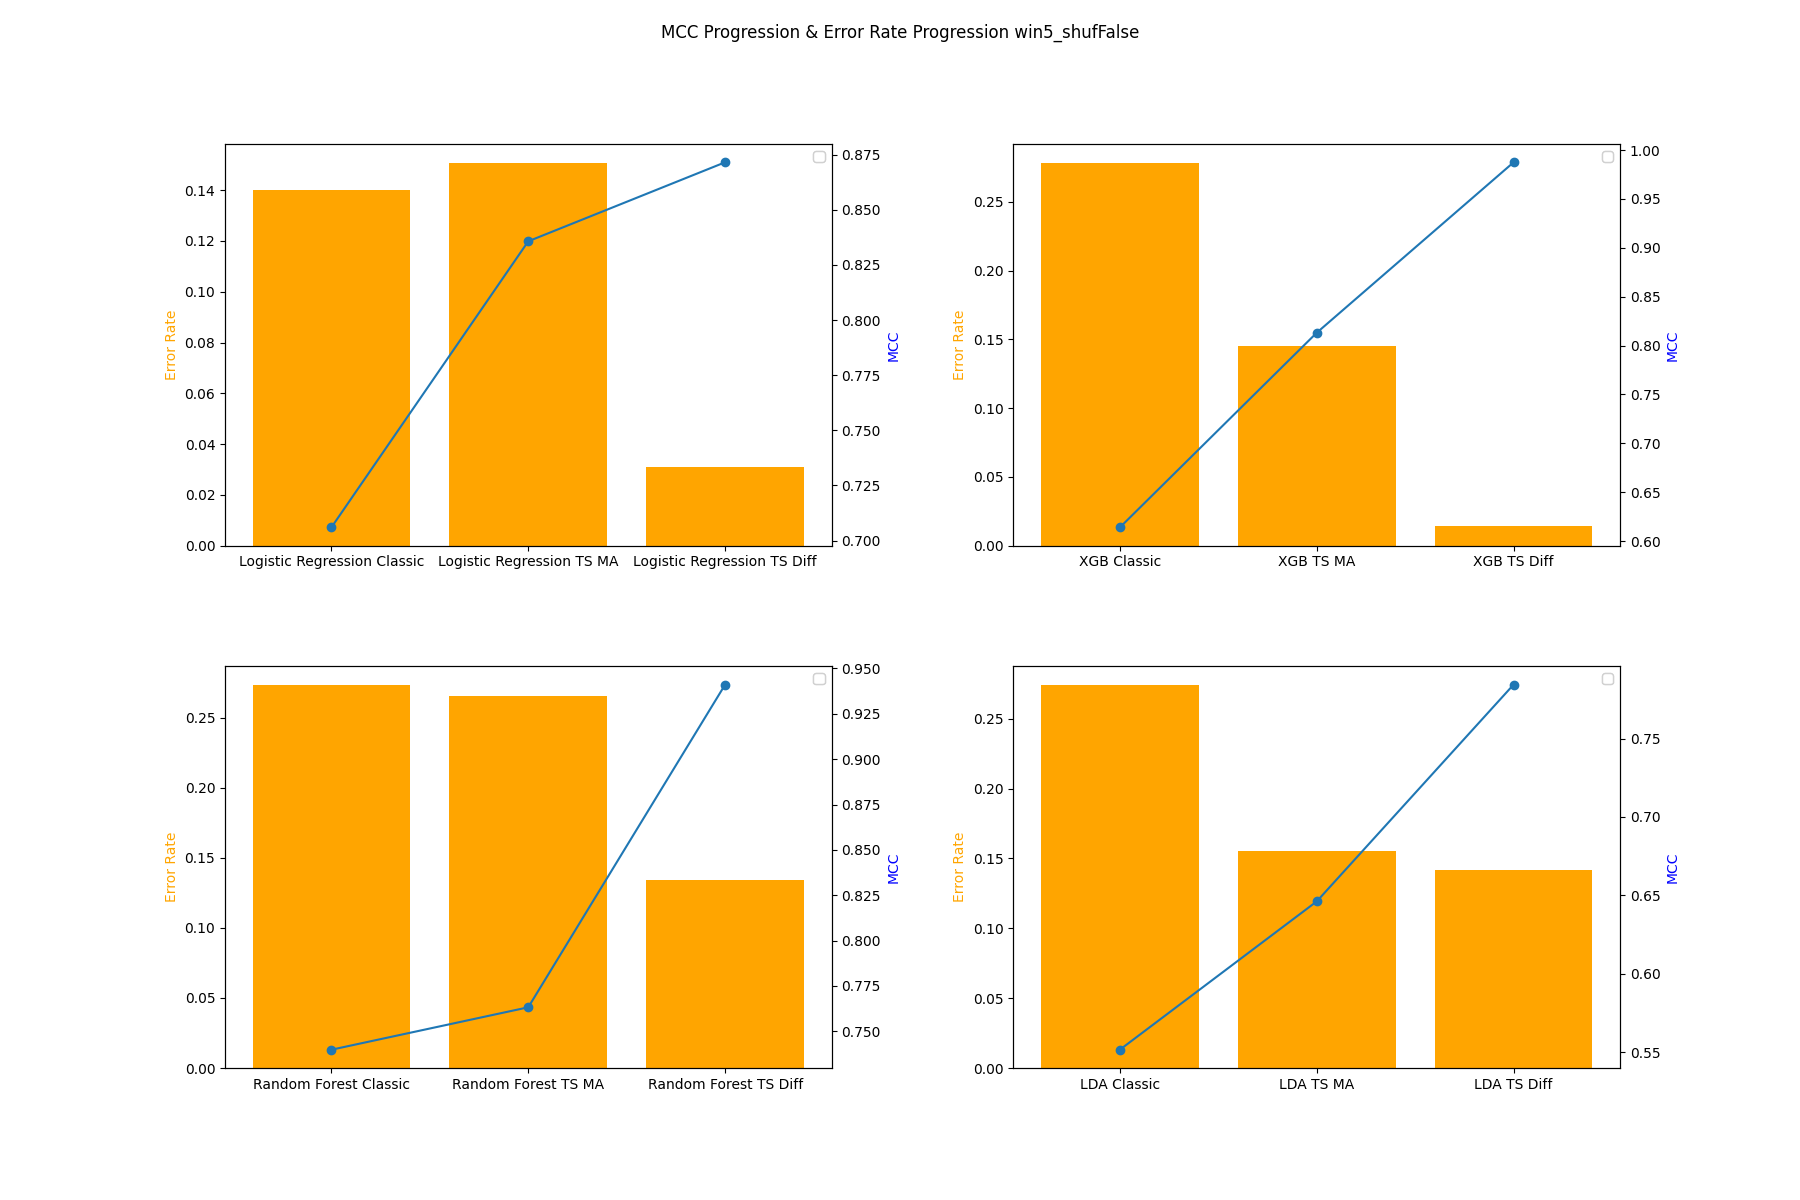
\includegraphics[width=0.8\textwidth]{MCC_Progression_win5_shufFalse.png}}
    \caption{Comparazione Progressione MCC shuffle = True/False}
    \label{fig:comparazione30}
\end{figure}

Come si pu\`o notare dai risultati ottenuti, i modelli addestrati con il parametro \textit{shuffle} impostato a \textit{True} ottengono performance migliori in termini di MCC. L'ipotesi da cui siamo partiti per spiegare questo fenomeno \`e che i modelli addestrati con \textit{shuffle = False} dessero troppa importanza a delle features "inaffidabili" e che quindi portassero a un decremento delle prestazioni dei modelli. Per verificare questa ipotesi sono stati rappresentati i grafici delle prime 20 features pi\`u importanti per ogni modello, ovvero quelle a cui veniva attirbuito maggior peso. A titolo di esempio vengono mostrate le feature importance per i modelli \textit{classic} XGBoost con \textit{window = 5}.

\begin{figure}[H]
    \centering
    \subfloat[Shuffle = True]{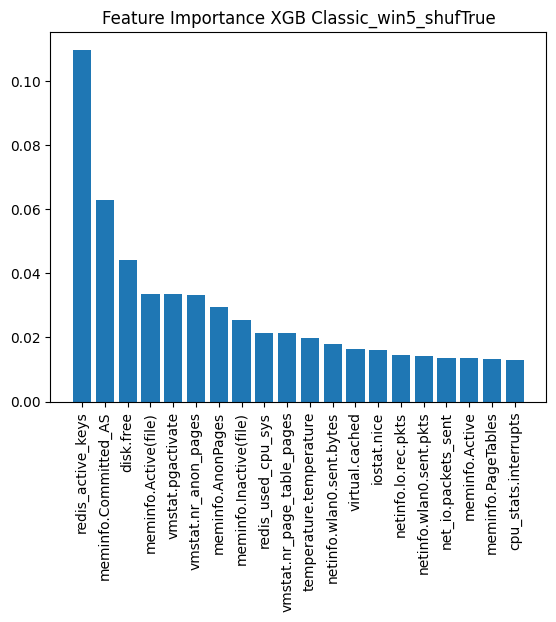
\includegraphics[width=0.5\textwidth]{Feature Importance XGB Classic_win5_shufTrue.png}}
    \hfill
    \subfloat[Shuffle = False]{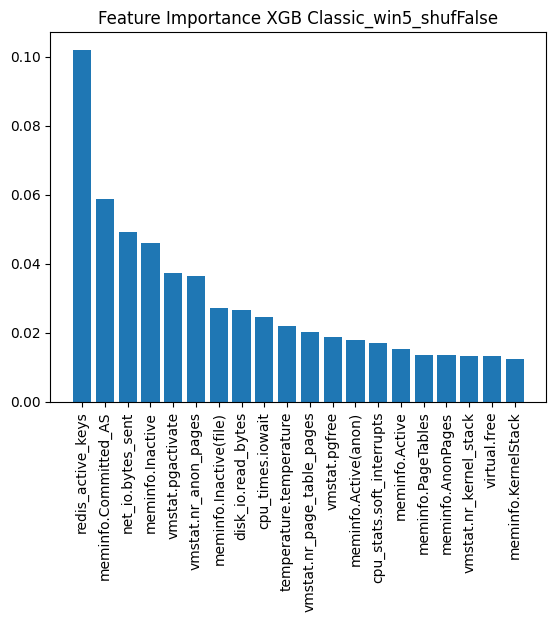
\includegraphics[width=0.5\textwidth]{Feature Importance XGB Classic_win5_shufFalse.png}}
    \caption{Comparazione Feature Importance XGBoost classic window = 5 shuffle = True/False}
    \label{fig:comparazione_feature}
\end{figure}

\vspace{0.5 cm}

Come volevasi dimostrare, le feature importance dei due modelli sono differenti. Ci sono alcune features in comune nella stessa posizione, altre in posizione diversa e altre ancora sono presenti in una e non nell'altra. Diamo ora la definizione di feature inaffidabile: feature non presente nel grafico (a) e presente nel grafico (b) o, anche se presente nel grafico (a), non in prossimit\`a della posizione individuata nel grafico (b)  \ref{fig:comparazione_feature}. Sono state quindi eliminate le feature inaffidabili dal dataset ed \`e stato eseguito nuovamente il training del modello con il parametro \textit{shuffle = False} sul nuovo dataset.
Questa operazione di eliminazione delle features inaffidabili \`e stata eseguita per ogni modello con approccio \textit{classic}, perch\'e si \`e dimostrato l'approccio con maggiore differenza in termini di MCC tra modelli addestrati con e senza \textit{shuffle}, come si vede nel grafico \ref{fig:comparazione30}. L'analisi delle feature inaffidabili \`e stata svolta solo sui modelli addestrati con approccio \textit{classic} , dato che il miglioramento pi\`u sensibile era previsto per questi modelli, ma un miglioramento \`e atteso anche per i modelli addestrati con approcci diversi. Infine i nuovi modelli sono stati testati sul datatset \textit{my-all3} ed \`e stata effettuata una comparazione con i vecchi modelli, in termini di MCC.

\begin{figure}[H]
    \centering
    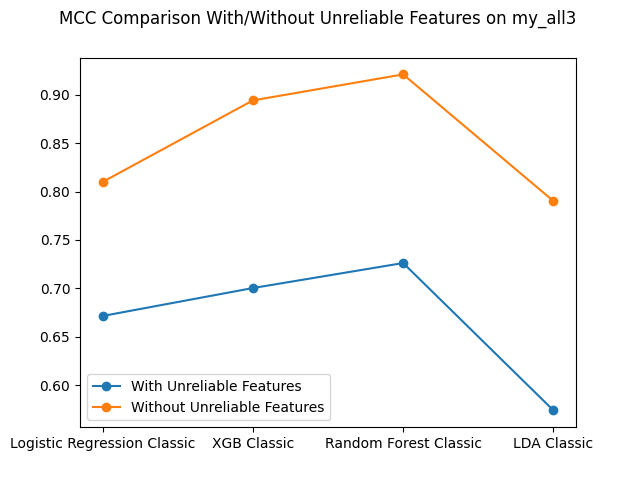
\includegraphics[width=0.78\linewidth]{MCC_Comparison_With_Without_Unreliable_Features_All3.png}
    \caption{Comparazione MCC modelli con e senza feature inaffidabili}
    \label{fig:enter-label}
\end{figure}

\vspace{0.5 cm}

Come si vede dal grafico riportato qui sopra, c'\`e un netto miglioramento delle performance da parte dei modelli che sono stati addestrati escludendo le feature inaffidabili.


 \vspace{-0.5cm}
 \vspace{-0.3cm}
